% This document is licensed under:
% Creative Commons NonCommercial-Attribution-ShareAlike
% 2020
% Author: Spacial
% spacial_AT@gmail_DOT_com
\documentclass[a4paper,12pt]{article} 
\usepackage[utf8]{inputenc}
\usepackage[T1]{fontenc}
\usepackage[brazil]{babel}
\usepackage{amsmath}
\usepackage{amsfonts}
\usepackage{amssymb} 
\usepackage{graphicx} 
\usepackage{hyperref} 
\hypersetup{pdfstartview = {XYZ null null 1.00}}
\usepackage[hmargin=2cm,vmargin=3cm]{geometry}
\usepackage{wrapfig}
\usepackage{enumitem}
\usepackage{fancyhdr}
\usepackage{float}
\usepackage{eurosym}
\usepackage{abnt}
\pagestyle{fancy}
\usepackage[printwatermark]{xwatermark}
\usepackage{lastpage}
\usepackage{graphicx}
\usepackage[
    type={CC},
    modifier={by-nc-sa},
    version={4.0},
]{doclicense}
\usepackage{fontawesome5}
\newcommand{\hsp}{\hspace{20pt}}
\newcommand{\HRule}{\rule{\linewidth}{0.5mm}}
\newwatermark[allpages,color=gray!5,angle=45,scale=3,xpos=0,ypos=0]{Regressão Linear\\ \texttt{CC by-nc-sa 4.0}}
\usepackage{listings}

\lstset{language=Rlang,
    basicstyle=\small\ttfamily,
    stringstyle=\color{red},
    otherkeywords={0,1,2,3,4,5,6,7,8,9},
    morekeywords={abbreviate,abline,abs,acos,acosh,action,add1,add,%
      aggregate,alias,Alias,alist,all,anova,any,aov,aperm,append,apply,%
      approx,approxfun,apropos,Arg,args,array,arrows,as,asin,asinh,%
      atan,atan2,atanh,attach,attr,attributes,autoload,autoloader,ave,%
      axis,backsolve,barplot,basename,besselI,besselJ,besselK,besselY,%
      beta,binomial,body,box,boxplot,break,browser,bug,builtins,bxp,by,%
      c,C,call,Call,case,cat,category,cbind,ceiling,character,char,%
      charmatch,check,chol,chol2inv,choose,chull,class,close,cm,codes,%
      coef,coefficients,co,col,colnames,colors,colours,commandArgs,%
      comment,complete,complex,conflicts,Conj,contents,contour,%
      contrasts,contr,control,helmert,contrib,convolve,cooks,coords,%
      distance,coplot,cor,cos,cosh,count,fields,cov,covratio,wt,CRAN,%
      create,crossprod,cummax,cummin,cumprod,cumsum,curve,cut,cycle,D,%
      data,dataentry,date,dbeta,dbinom,dcauchy,dchisq,de,debug,%
      debugger,Defunct,default,delay,delete,deltat,demo,de,density,%
      deparse,dependencies,Deprecated,deriv,description,detach,%
      dev2bitmap,dev,cur,deviance,off,prev,,dexp,df,dfbetas,dffits,%
      dgamma,dgeom,dget,dhyper,diag,diff,digamma,dim,dimnames,dir,%
      dirname,dlnorm,dlogis,dnbinom,dnchisq,dnorm,do,dotplot,double,%
      download,dpois,dput,drop,drop1,dsignrank,dt,dummy,dump,dunif,%
      duplicated,dweibull,dwilcox,dyn,edit,eff,effects,eigen,else,%
      emacs,end,environment,env,erase,eval,equal,evalq,example,exists,%
      exit,exp,expand,expression,External,extract,extractAIC,factor,%
      fail,family,fft,file,filled,find,fitted,fivenum,fix,floor,for,%
      For,formals,format,formatC,formula,Fortran,forwardsolve,frame,%
      frequency,ftable,ftable2table,function,gamma,Gamma,gammaCody,%
      gaussian,gc,gcinfo,gctorture,get,getenv,geterrmessage,getOption,%
      getwd,gl,glm,globalenv,gnome,GNOME,graphics,gray,grep,grey,grid,%
      gsub,hasTsp,hat,heat,help,hist,home,hsv,httpclient,I,identify,if,%
      ifelse,Im,image,\%in\%,index,influence,measures,inherits,install,%
      installed,integer,interaction,interactive,Internal,intersect,%
      inverse,invisible,IQR,is,jitter,kappa,kronecker,labels,lapply,%
      layout,lbeta,lchoose,lcm,legend,length,levels,lgamma,library,%
      licence,license,lines,list,lm,load,local,locator,log,log10,log1p,%
      log2,logical,loglin,lower,lowess,ls,lsfit,lsf,ls,machine,Machine,%
      mad,mahalanobis,make,link,margin,match,Math,matlines,mat,matplot,%
      matpoints,matrix,max,mean,median,memory,menu,merge,methods,min,%
      missing,Mod,mode,model,response,mosaicplot,mtext,mvfft,na,nan,%
      names,omit,nargs,nchar,ncol,NCOL,new,next,NextMethod,nextn,%
      nlevels,nlm,noquote,NotYetImplemented,NotYetUsed,nrow,NROW,null,%
      numeric,\%o\%,objects,offset,old,on,Ops,optim,optimise,optimize,%
      options,or,order,ordered,outer,package,packages,page,pairlist,%
      pairs,palette,panel,par,parent,parse,paste,path,pbeta,pbinom,%
      pcauchy,pchisq,pentagamma,persp,pexp,pf,pgamma,pgeom,phyper,pico,%
      pictex,piechart,Platform,plnorm,plogis,plot,pmatch,pmax,pmin,%
      pnbinom,pnchisq,pnorm,points,poisson,poly,polygon,polyroot,pos,%
      postscript,power,ppoints,ppois,predict,preplot,pretty,Primitive,%
      print,prmatrix,proc,prod,profile,proj,prompt,prop,provide,%
      psignrank,ps,pt,ptukey,punif,pweibull,pwilcox,q,qbeta,qbinom,%
      qcauchy,qchisq,qexp,qf,qgamma,qgeom,qhyper,qlnorm,qlogis,qnbinom,%
      qnchisq,qnorm,qpois,qqline,qqnorm,qqplot,qr,Q,qty,qy,qsignrank,%
      qt,qtukey,quantile,quasi,quit,qunif,quote,qweibull,qwilcox,%
      rainbow,range,rank,rbeta,rbind,rbinom,rcauchy,rchisq,Re,read,csv,%
      csv2,fwf,readline,socket,real,Recall,rect,reformulate,regexpr,%
      relevel,remove,rep,repeat,replace,replications,report,require,%
      resid,residuals,restart,return,rev,rexp,rf,rgamma,rgb,rgeom,R,%
      rhyper,rle,rlnorm,rlogis,rm,rnbinom,RNGkind,rnorm,round,row,%
      rownames,rowsum,rpois,rsignrank,rstandard,rstudent,rt,rug,runif,%
      rweibull,rwilcox,sample,sapply,save,scale,scan,scan,screen,sd,se,%
      search,searchpaths,segments,seq,sequence,setdiff,setequal,set,%
      setwd,show,sign,signif,sin,single,sinh,sink,solve,sort,source,%
      spline,splinefun,split,sqrt,stars,start,stat,stem,step,stop,%
      storage,strstrheight,stripplot,strsplit,structure,strwidth,sub,%
      subset,substitute,substr,substring,sum,summary,sunflowerplot,svd,%
      sweep,switch,symbol,symbols,symnum,sys,status,system,t,table,%
      tabulate,tan,tanh,tapply,tempfile,terms,terrain,tetragamma,text,%
      time,title,topo,trace,traceback,transform,tri,trigamma,trunc,try,%
      ts,tsp,typeof,unclass,undebug,undoc,union,unique,uniroot,unix,%
      unlink,unlist,unname,untrace,update,upper,url,UseMethod,var,%
      variable,vector,Version,vi,warning,warnings,weighted,weights,%
      which,while,window,write,\%x\%,x11,X11,xedit,xemacs,xinch,xor,%
      xpdrows,xy,xyinch,yinch,zapsmall,zip,TRUE,FALSE},%
    otherkeywords={!,!=,~,\$,*,\&,\%/\%,\%*\%,\%\%,<-,<<-,_,/},%
    deletekeywords={data,frame,length,as,character},
    keywordstyle=\color{blue},
    otherkeywordstyle=\color{red},
    commentstyle=\color{gray},
}

\usepackage[dvipsnames, svgnames]{xcolor}


\begin{document}
\begin{titlepage}
  \begin{sffamily}
  \begin{center}
  \vspace{5cm}

    % Title
    \HRule \\[0.4cm]
    { \huge \bfseries Atividade Final de Estatística \\[0.4cm] }
    
    \HRule \\[2cm]

    \textsc{\LARGE Matéria: Inferência Estatística}\\[1cm]
    \begin{minipage}{0.4\textwidth}
      \begin{flushleft} \large
		\emph{Equipe :} \\        
        \textsc{Spacial}\\
      \end{flushleft}
    \end{minipage}
    \begin{minipage}{0.4\textwidth}
      \begin{flushright} \large
        \textsc{Brasil} 
      \end{flushright}
    \end{minipage}

    \vfill

    % Bottom of the page
    {\large Pós-Graduação em \textit{DataScience}}

  \end{center}
  \end{sffamily}
  \doclicenseThis
\end{titlepage}
\newpage

%HEADER
\renewcommand{\headrulewidth}{1pt}
\fancyhead[R]{\small Este trabalho está licenciado sob \texttt{CC-BY-SA 4.0} \faCreativeCommons\ \faCreativeCommonsBy\ \faCreativeCommonsSa}
\fancyfoot[C]{\thepage/\pageref{LastPage}}
\fancyhead[L]{Atividade Final}
{\ \vspace{-0.51cm}}

\tableofcontents

\section{Atividade Inferência e Hipótese}

\subsection{Informações Gerais}

Informe o método utilizado e justifique. A formulação da resposta faz parte da avaliação. Exibir o código utilizado no R.

\subsection{Exercícios}

\begin{enumerate}
    \item A empresa fictícia TI Systems utiliza o tempo de ponto de função para estimar o custo de um sistema.\newline
    É considerado 2 horas como o custo de mão de obra por medida. Sabe-se que o desvio padrão é de 0,5 hora. \newline
    No mês passado os tempos por ponto de função coletados foram de:
    \begin{center}
\texttt{1,9  1,7  2,8  2,4  2,6  2,5  2,8  3,2  1,6  2,5} \\
    \end{center}
    Usando p=0,05, verifique se o custo excede 2 horas. \\
    \textbf{Pergunta}: Qual é sua conclusão e que recomendações você consideraria fazer aos gerentes? 
    \begin{itemize}
        \item \textbf{Código}:
        \begin{lstlisting}[language=Rlang]
amostra <- c(1.9, 1.7, 2.8, 2.4, 2.6, 2.5, 2.8, 3.2, 1.6, 2.5)
sigma <- sd(amostra)
N <- length(amostra)
med <- mean(amostra)
conf <- 0.95
gl <- N -1
Tc <- qt(0.975,lower.tail = T, df= gl)
IC <- c(med - Tc * sigma/sqrt(N),med + Tc* sigma/sqrt(N))
IC
        \end{lstlisting}
        \item \textbf{Resposta}:\\
        Com o intervalo de confiança de 95\% ficando entre: \texttt{2.0306 <-> 2.7694},
        tem-se que o custo real está maior que o custo estimado (\textit{2 horas}). Com isso sugere-se que o cálculo de custo de pontos por função seja alterado para mais próximo da média (e aí o apetite ao risco dos mesmo) ou que seja melhorada a mão de obra (para executar os pontos de função com menor quantidade de horas).
    \end{itemize}
    \item Uma indústria testa a aplicação de uma nova liga metálica na fabricação de seus produtos. Analisa-se a resistência de 7 linhas de produtos distintas. \textbf{Há aumento da resistência dos produtos ao adotar o metal 2?} Utilize $90\%$ de confiança. 
    \begin{center}
        \begin{tabular}{c|c|c}
        \textbf{Marca} &\textbf{ Metal 1} & \textbf{Metal 2} \\
        \hline
        A & 68 & 61  \\
        \hline
        B & 75 & 69 \\
        \hline
        C  &  62 & 64 \\
        \hline
        D  & 86 & 76 \\
        \hline
        E & 52 & 52 \\
        \hline
        F & 46 & 38 \\
        \hline
        G & 72 &  68\\
        \end{tabular}
    \end{center}
    \begin{itemize}
        \item \textbf{Código}:
                \begin{lstlisting}
# amostras
metal1 = c(68,75,62,86,52,46,72)
metal2 = c(61,69,64,76,52,38,68)
# tamanho de N é igual, confiança e graus de liberdade
N <- length(metal1)
conf <- 0.90
gl <- N-1
# amostra metal 1
med1 <- mean(metal1)
sigma1 <- sd(metal1)
Tc1 <- qt(0.95,lower.tail=T, df=gl)
IC1 <- c(med1 - Tc1*sigma1/sqrt(N), 
         med1 + Tc1*sigma1/sqrt(N))
IC1
# amostra metal 2
med2 <- mean(metal2)
sigma2 <- sd(metal2)
Tc2 <- qt(0.95,lower.tail=T, df=gl)
IC2 <- c(med2 - Tc2*sigma2/sqrt(N), 
         med2 + Tc2*sigma2/sqrt(N))
IC2
                \end{lstlisting}
        \item \textbf{Resposta}:\\
        Conforme observa-se, os intervalos de confiança (com 90\%) das amostras são: \textit{metal 1} \texttt{55.7652 <-> 75.9491} e \textit{metal 2} \texttt{51.8679 <-> 70.4178}.
        Conclui-se que não há aumento da resistência dos produtos ao adotar o \textbf{metal 2}, já que o intervalo mostrou que a resistência ficou menor.
    \end{itemize}
    \item Uma linha de produção tem os seguintes pesos em $kg$:
    \begin{verbatim}
5.4, 4.5, 4.7, 4.0, 3.9, 5.3, 5.4, 5.1, 5.9, 7.1, 4.5, 2.7,
6.0, 4.3, 4.3, 6.0, 4.7, 3.8, 5.2, 4.9, 5.0, 5.4, 4.6, 5.6, 
4.8, 5.3, 6.1, 5.4, 4.7, 6.1, 6.0, 5.5, 5.2, 4.4, 6.4, 4.4,
7.2, 6.5, 4.8, 4.0
    \end{verbatim} Calcule no R:
    \begin{itemize}
        \item[\textbf{A)}] Mediana:
            \begin{itemize}
                \item \textbf{Código}:
                \begin{lstlisting}
prod <- c(5.4, 4.5, 4.7, 4.0, 3.9, 5.3, 5.4, 
5.1, 5.9, 7.1, 4.5, 2.7, 6.0, 4.3, 4.3, 6.0, 
4.7, 3.8, 5.2, 4.9, 5.0, 5.4, 4.6, 5.6, 4.8, 
5.3, 6.1, 5.4, 4.7, 6.1, 6.0, 5.5, 5.2, 4.4, 
6.4, 4.4, 7.2, 6.5, 4.8, 4.0)
summary(prod)
                \end{lstlisting}
                \item \textbf{Resposta}:  \textbf{$5.150$}
            \end{itemize}  
        \item[\textbf{B)}] Média:
            \begin{itemize}
                \item \textbf{Código}:
                \begin{lstlisting}
summary(prod)
                \end{lstlisting}
                \item \textbf{Resposta}:  \textbf{$5.128$}
            \end{itemize}
        \item[\textbf{C)}] Desvio Padrão:
            \begin{itemize}
                \item \textbf{Código}:
                \begin{lstlisting}
sd(prod)
                \end{lstlisting}
                \item \textbf{Resposta}:  \textbf{$0.9229$}
            \end{itemize}
        \item[\textbf{D)}] Calcule o 1o quartil, 2o quartil e 3o quartil:
            \begin{itemize}
                \item \textbf{Código}:
                \begin{lstlisting}
summary(prod)
                \end{lstlisting}
                \item \textbf{Resposta}: $ $ $1^{o}Q: 4.5$ / $2^{o}Q: 5.15$ / $3^{o}Q: 5.675$ 
            \end{itemize}
        \item[\textbf{E)}] Plote o \textit{boxplot} (diagrama de caixa) da amostra:
            \begin{itemize}
                \item \textbf{Código}:
                \begin{lstlisting}
boxplot(prod)
                \end{lstlisting}
                \item \textbf{Resposta}: % Figura \ref{figbox}
                    \begin{figure}[h!tb]
                     \centering
                     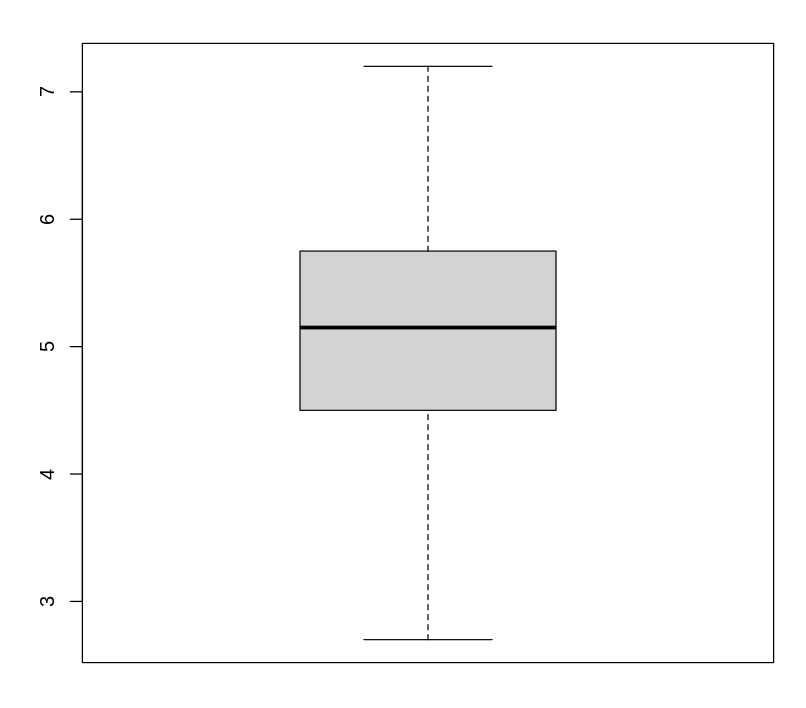
\includegraphics[scale=0.45]{1_3e_boxplot.png}
                     \caption{BoxPlot.}
                     \label{figbox}
                    \end{figure}
            \end{itemize}
        \item[\textbf{F)}] Plote o histograma da amostra:
            \begin{itemize}
                \item \textbf{Código}:
                \begin{lstlisting}
hist(prod)
                \end{lstlisting}
                \item \textbf{Resposta}: %Figura \ref{fighist}
                    \begin{figure}[h!tb]
                     \centering
                     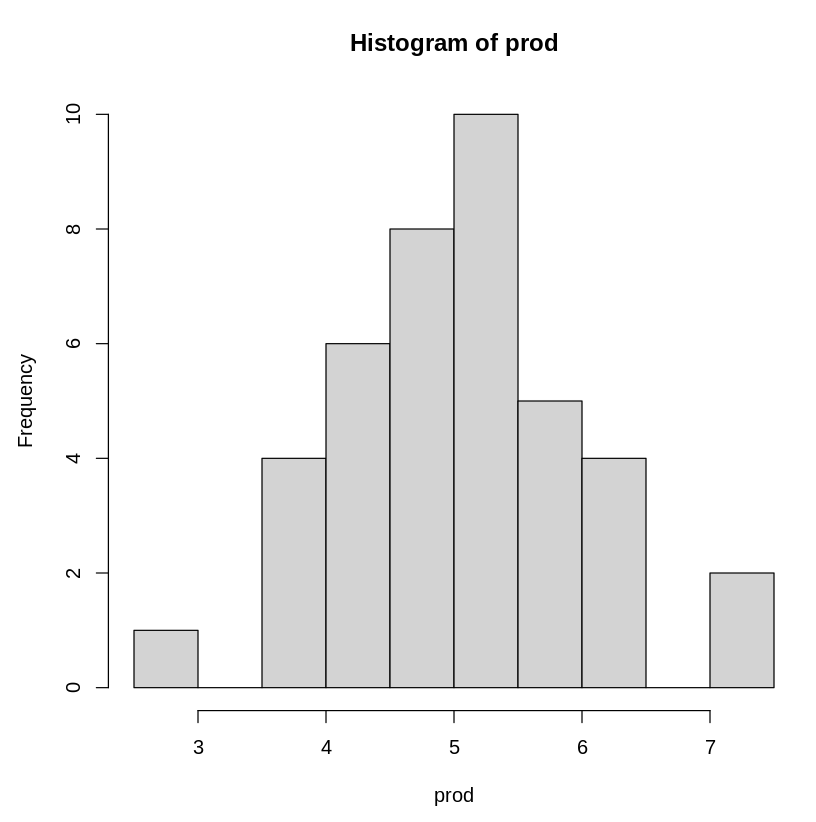
\includegraphics[scale=0.45]{1_3f_hist.png}
                     \caption{Histrograma.}
                     \label{fighist}
                    \end{figure}
            \end{itemize}
        \item[\textbf{G)}] qual a probabilidade um produto ter um peso entre $4.2$ e $5.2$?
            \begin{itemize}
                \item \textbf{Código}:
                \begin{lstlisting}
# p > 4.2 e p < 5.2
Z4 <- (4.2-mean(prod))/sd(prod)
Z5 <- (5.2-mean(prod))/sd(prod)
prob <- pnorm(Z5) - pnorm(Z4)
round(prob,4)
                \end{lstlisting}
                \item \textbf{Resposta}: A probabilidade de ficar entre $4.2$ e $5.2$ é de $37.38\%$.
            \end{itemize}
    \end{itemize}
\end{enumerate}

\section{Atividade Regressões Lineares}

\subsection{Informações Gerais}

Informe o método utilizado e justifique. A formulação da resposta faz parte da avaliação. Exibir o código utilizado no R.

\subsection{Exercícios}

\subsubsection{Exercício 1}

\begin{enumerate}
    \item Faça a análise conforme descrito a seguir:
    \begin{enumerate}
        \item[1.1] Defina a renda média \textit{per-capita} do estado em relação a média de escolaridade do estado (y = renda, x = escolaridade) em outras palavras renda $\sim$ escolaridade) dos dados públicos a seguir:
            \begin{lstlisting}
#dados para o exercicio copie e cole no R

mec <-  data.frame(  
row.names  =    c("RR", "AC", "PA", "TO", "MA", "SE", "BA", 
"AL", "SP", "ES", "SC", "PR", "GO", "DF", "AP", "RO", "AM", 
"PB", "RN", "PI", "PE", "CE", "RJ", "MG", "RS", "MT", "MS"),
  
escolaridade = c(5.7, 4.5, 4.7, 4.5, 3.6, 4.3, 4.1, 3.7, 6.8,
5.7, 6.3, 6.0, 5.5, 8.2, 6.0, 4.9, 5.5, 3.9, 4.5, 3.5, 4.6, 
4.0, 7.1, 5.4, 6.4, 5.4, 5.7),
  
renda =  c(685, 526, 536, 520, 343, 462, 460, 454, 1076, 722, 
814, 782, 689, 1499, 683, 662, 627, 423, 513, 383, 517, 448, 
970, 681, 800, 775, 731)
)
            \end{lstlisting}
        \item[1.2] Veja os gráficos de dispersão: Figura \ref{fig2disp}.\\
        \textbf{Código}:
            \begin{lstlisting}
ggplot(mec,aes(x=escolaridade, y=renda, 
           color=(renda/escolaridade))) +
geom_point(shape = 16, size = 5, show.legend = FALSE) +
theme_minimal()
            \end{lstlisting}
            \begin{figure}[h!tb]
             \centering
             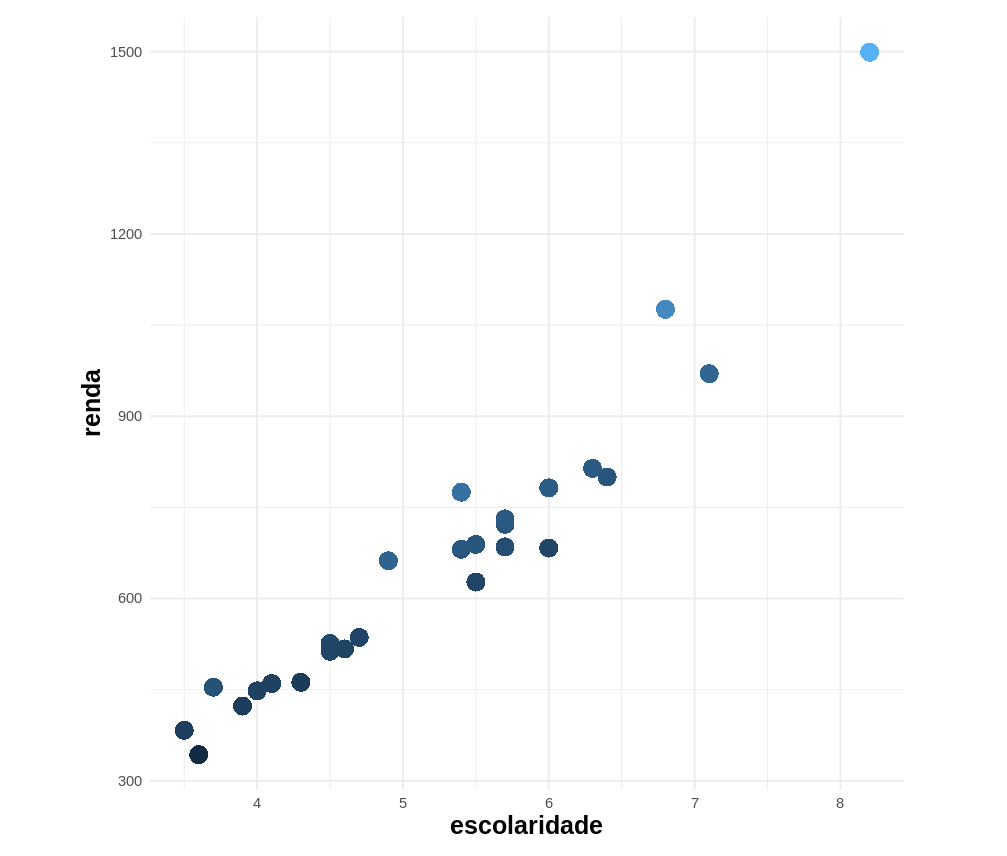
\includegraphics[scale=0.45]{2_1a_scatter.png}
             \caption{Gráfico de Dispersão.}
             \label{fig2disp}
            \end{figure}
        \item[1.3] Exiba as correlações:\\
        \textbf{Código}:
            \begin{lstlisting}
correlacao <- cor(escolaridade,renda)
            \end{lstlisting}
            \textbf{Resposta}:   correlação direta forte: $0.9507$
        \item[1.4] Plote os histogramas de renda e escolaridade: \\
            \textbf{Código}:
                \begin{lstlisting}
par(
  mfrow=c(1,2),
  mar=c(4,4,1,0)
) 
hist(mec$escolaridade, breaks=5 , ylim=c(0,12), 
      col="#e6b9b3" , xlab="escolaridade" , 
      ylab="", main="") 
hist(mec$renda, breaks=5, ylim=c(0,12), 
       xlab="renda" , ylab="", main="",
        col="#b3cce6")  
                \end{lstlisting}
                \textbf{Resposta}:  Figura \ref{fig2hist}
                \begin{figure}[h!tb]
                     \centering
                     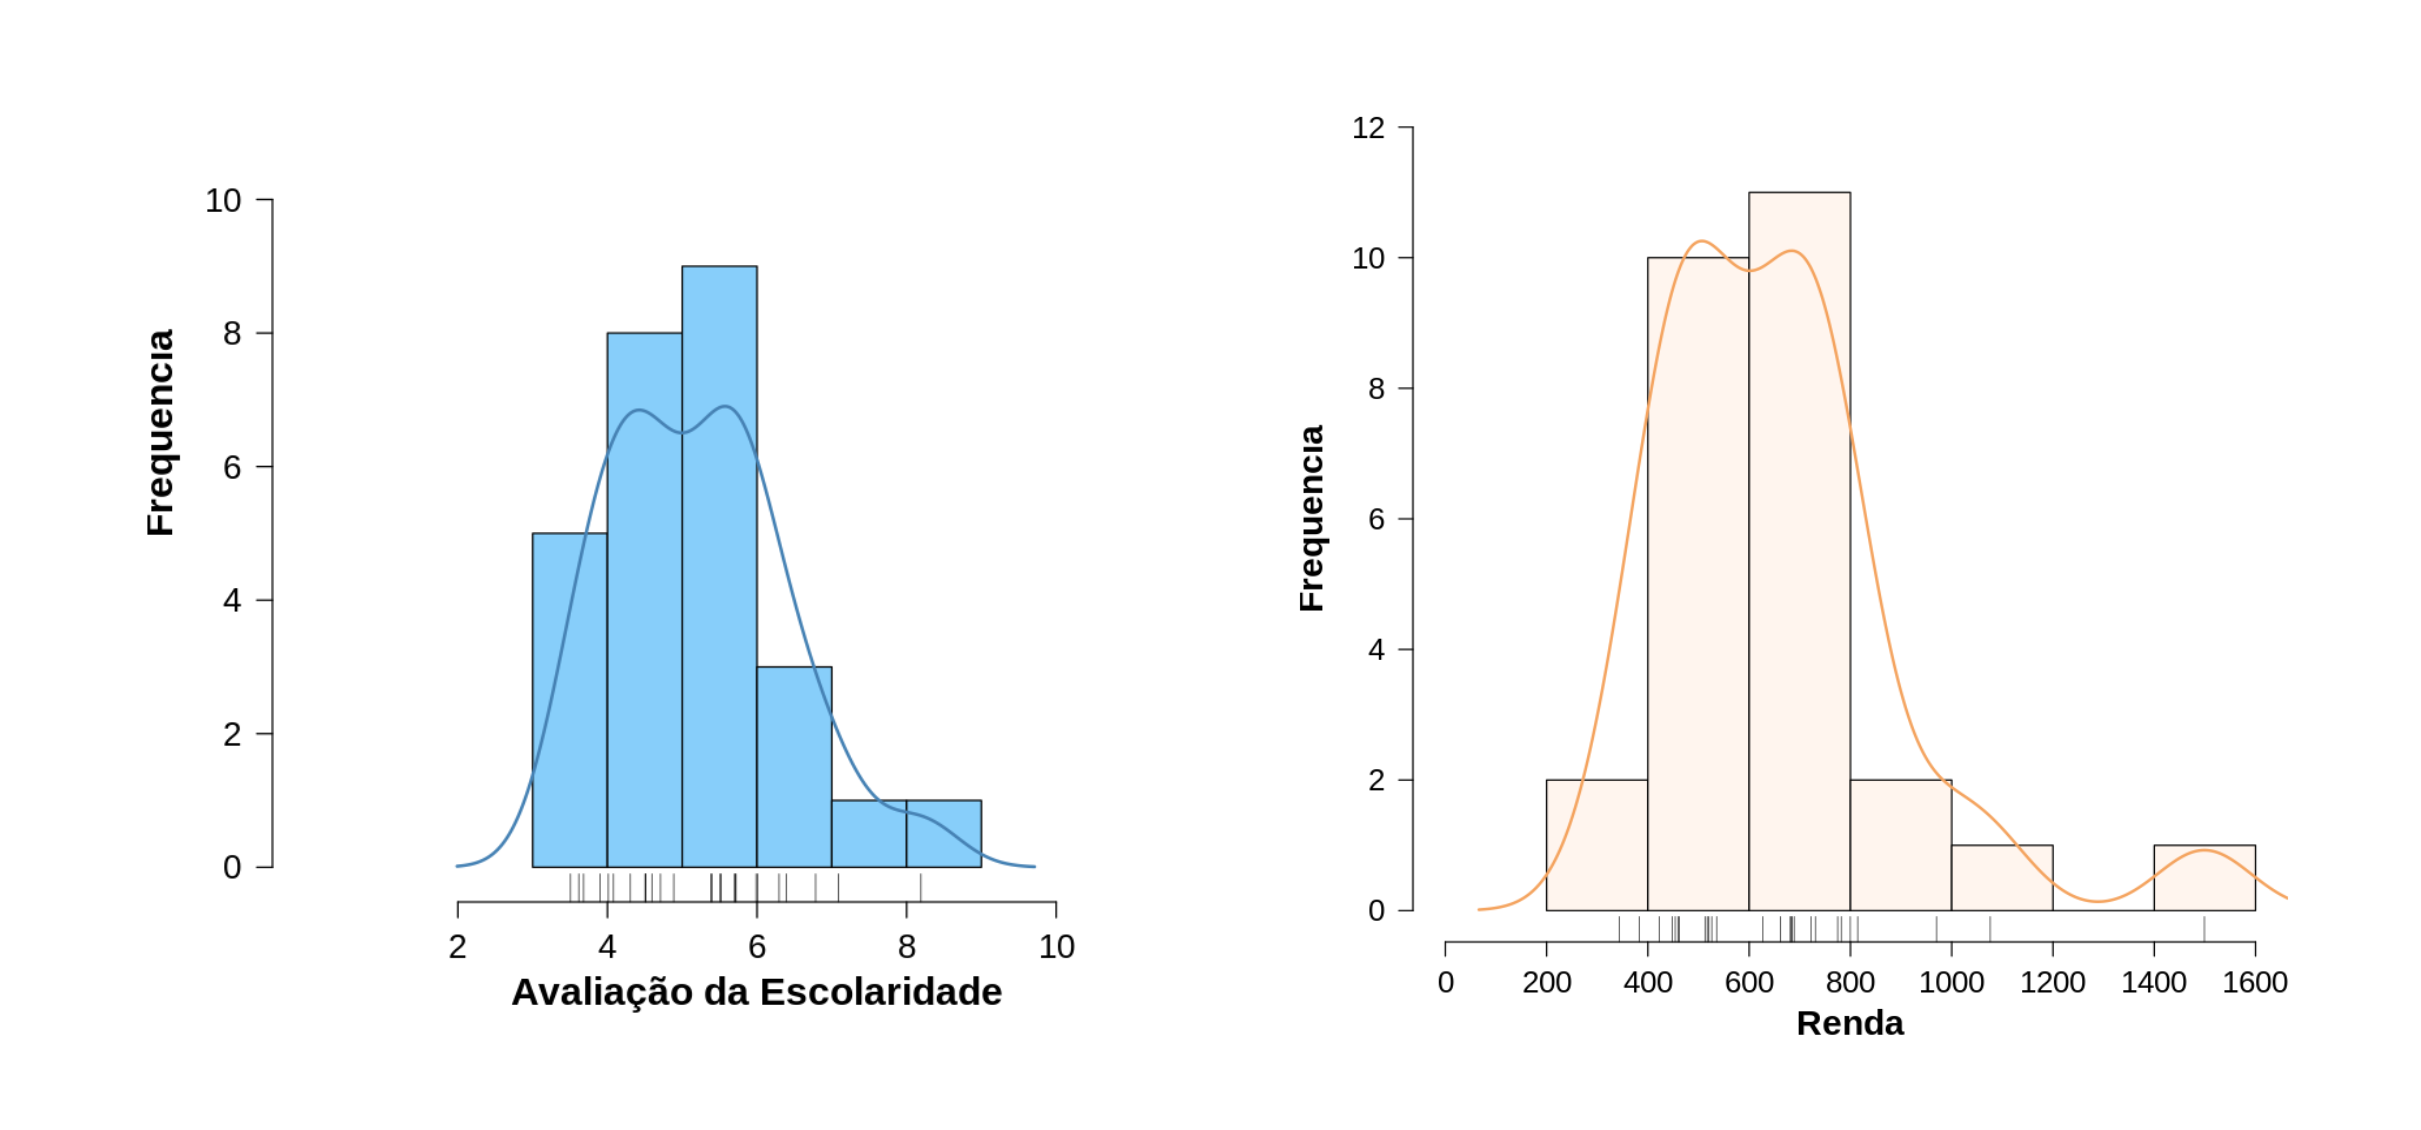
\includegraphics[scale=0.4]{2_1b_hist.png}
                     \caption{Histogramas das variáveis com a linha de dispersão.}
                     \label{fig2hist}
                \end{figure}
        \item[1.5] Teste de normalidade: \\
        \textbf{Código}:
            \begin{lstlisting}
shapiro.test(renda)$p.value
shapiro.test(escolaridade)$p.value
fligner.test(renda ~ escolaridade, mec)
            \end{lstlisting}
            \textbf{Resposta}:  No caso do teste de \textit{Shapiro} em cada conjunto de dados (renda e escolaridade), o primeiro ficou menor que \textit{0.05}, mostrando que os dados não seguem uma distribuição normal. Já no caso da escolaridade, os dados seguem. \\
            No teste de \textit{Fligner}, o valor foi \texttt{p-value = 0.2153}, nos indicando que há igualdade entre as variâncias.
        \item[1.6] Faça a regressão linear \texttt{lm()}:\\
        \textbf{Código}:
            \begin{lstlisting}
modelo.linear <- lm (escolaridade ~ renda, mec)
coefficients(modelo.linear)
ggplot(mec,aes(x=renda, y=escolaridade, 
          color=(renda/escolaridade)), 
          show.legend = FALSE) +
       geom_point(shape = 16, size = 5, 
           show.legend = FALSE) +
       theme_minimal() + 
       geom_smooth(method = "lm", se = FALSE, 
       show.legend = FALSE) 
            \end{lstlisting}
            \textbf{Resposta}: Figura \ref{fig2lm}
                \begin{figure}[h!tb]
                     \centering
                     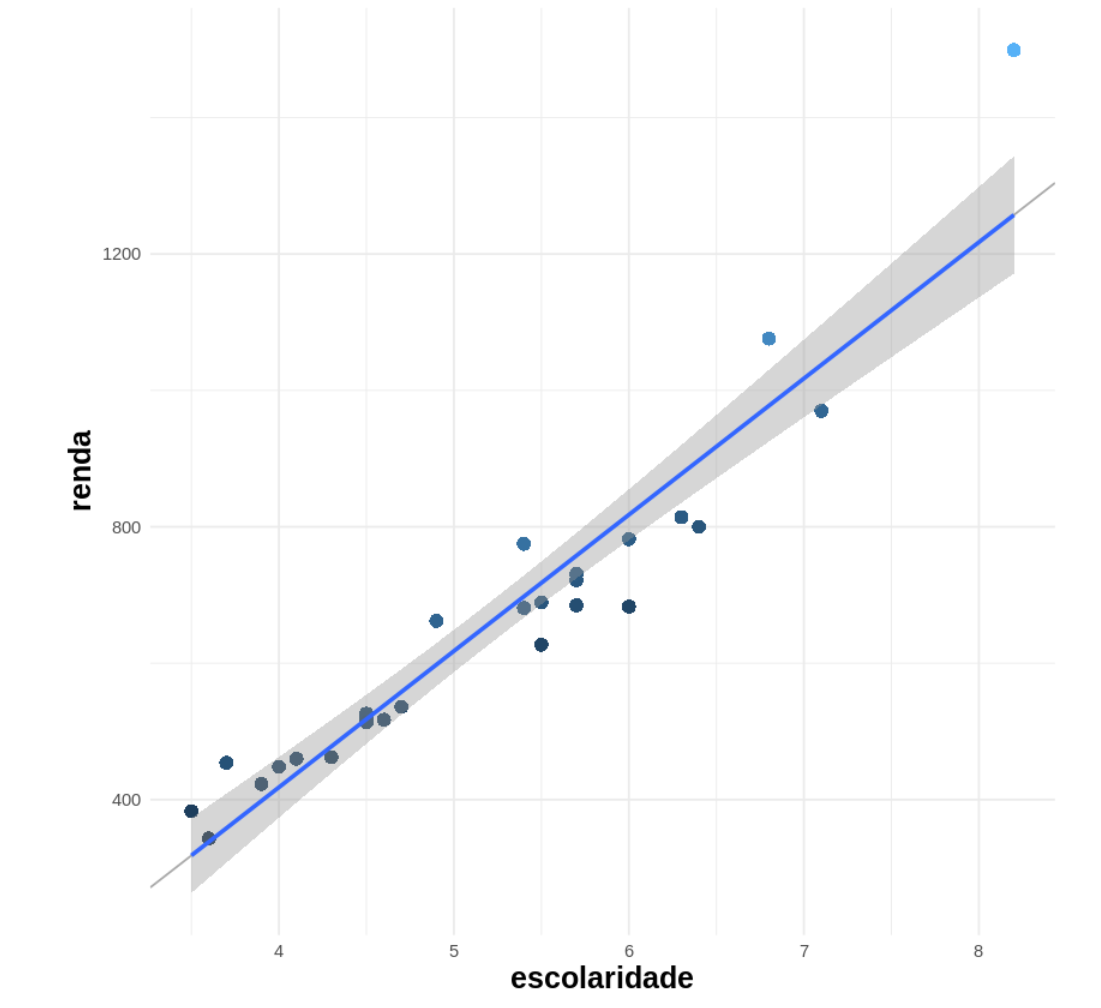
\includegraphics[scale=0.45]{2_1d_lm.png}
                     \caption{Regressão Linear Simples.}
                     \label{fig2lm}
                \end{figure}
        \item[1.7] Quais são os pontos com maior alavancagem? \\
        \textbf{Código}:
            \begin{lstlisting}
sort(influence(modelo.linear)$hat, decreasing = TRUE)[1:4]
            \end{lstlisting}
            \textbf{Resposta}: \texttt{DF}, \texttt{RJ}, \texttt{PI} e \texttt{MA}.
        \item[1.8] Qual o coeficiente de determinação (R-squared)? \\
        \textbf{Código}:
            \begin{lstlisting}
summary(modelo.linear)$r.squared
            \end{lstlisting}
            \textbf{Resposta}: Coeficiente de determinação: $0.9039$, isso nos indica que o modelo (a reta) explica $90\%$ da variação dos dados.
        \item[1.9] Verifique os resíduos com a biblioteca \texttt{library(hnp)} \\
        \textbf{Código}:
            \begin{lstlisting}
fit <- hnp(modelo.linear, print.on=TRUE, plot=FALSE)
plot(fit)
            \end{lstlisting}
                \textbf{Resposta}: Figura \ref{fig2res}.
                \begin{figure}[h!tb]
                     \centering
                     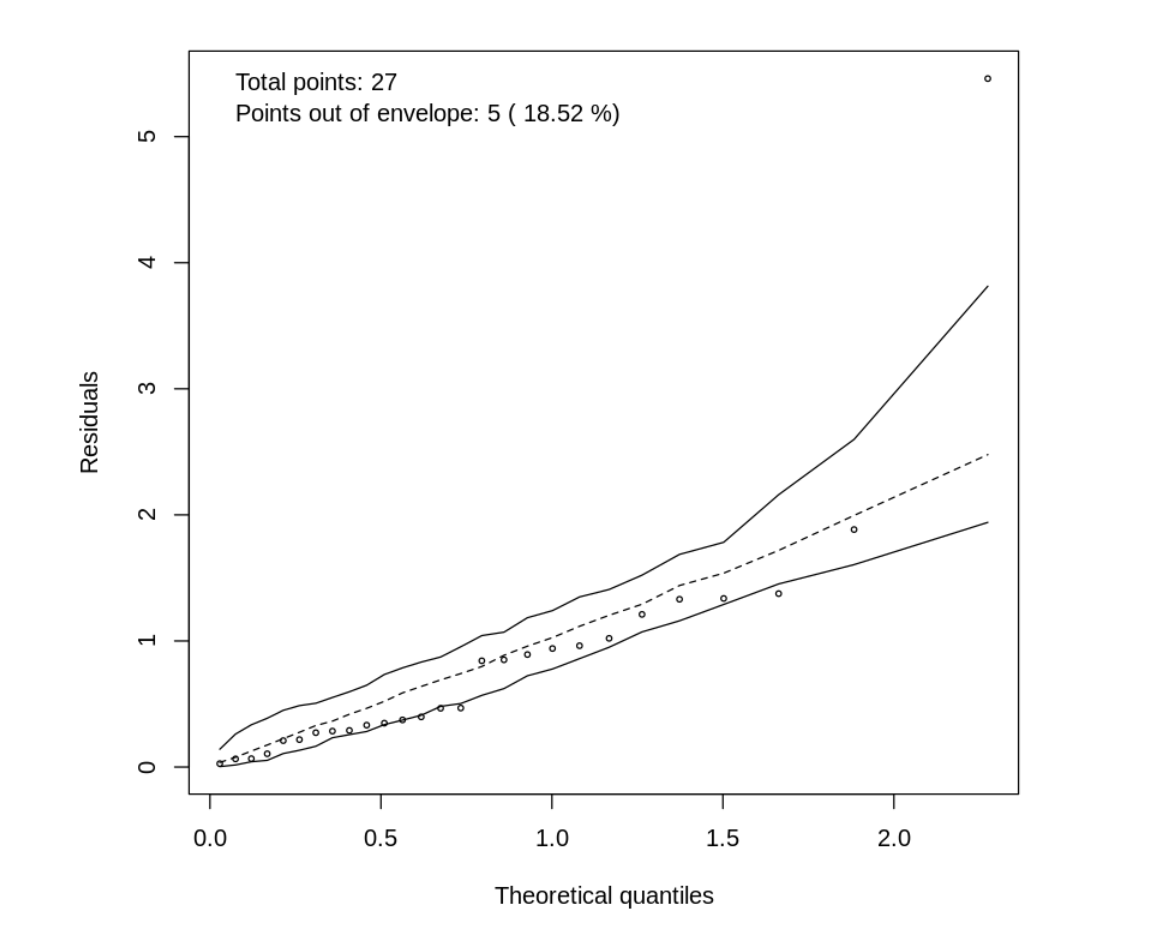
\includegraphics[scale=0.45]{2_1e_res.png}
                     \caption{Resíduos via biblioteca \texttt{hnp} aplicada ao modelo linear.}
                     \label{fig2res}
                \end{figure}
        \item[1.10] A regressão linear parece ser uma boa escolha? Por que? \\
              \textbf{Resposta}: Como visto na Figura \ref{fig2res}, o modelo linear deixa 5 pontos fora do intervalo ($18.5\%$). Ideal seriam que todos os pontos estivessem dentro do intervalo (mesmo \texttt{DF} que é um $outlier$).
        \item[1.11] Qual das distribuições que estudamos (Binomial, Normal, Poisson, Gama, Gaussiana Inversa) tem uma semelhança com os dados mostrados pelo histograma de renda?  \\
        \textbf{Resposta}: $Gamma$
        \item[1.12] Faça uma regressão \texttt{glm()} com essa distribuição \\
        \textbf{Código}:
            \begin{lstlisting}
modelo.glm <- glm(renda ~ escolaridade, data=mec, 
                      family = Gamma() )
ggplot(mec,aes(x=escolaridade, y=renda, bins=4,
       color=abs(renda-modelo.linear$fitted.values)), 
       breaks=1:8, ylim=c(200,1600), xlim=c(2,9), 
       show.legend = FALSE) +
  geom_smooth(method = "glm", show.legend = FALSE) + 
  geom_point(shape = 16, size = 4, 
               show.legend = FALSE, bins=5) +  
  geom_point(aes(x= escolaridade, 
                 y=modelo.linear$fitted.values), 
                 col = "firebrick4", size=3, 
                 pch = 18, alpha=0.5)+
  geom_abline(intercept = reta[1], slope=reta[2], 
                    col="goldenrod3") +
  geom_segment(aes(xend = escolaridade, 
                   yend = modelo.linear$fitted.values),
                   show.legend = FALSE, bins=5) + 
  theme_minimal() +
  theme(axis.title = element_text(color="black", 
          size=15, face=2))+
  scale_color_viridis() +
  ggtitle("Modelo GLM")
            \end{lstlisting}
            \textbf{Resposta}: Figura \ref{fig2glm} (nota\footnote{As cores dos pontos e segmentos representam a diferença entre a reta e valor do ponto em si, sendo o mais distante em amarelo e o mais próximo no roxo. Em vermelho, os pontos projetados.}):
                \begin{figure}[h!tb]
                     \centering
                     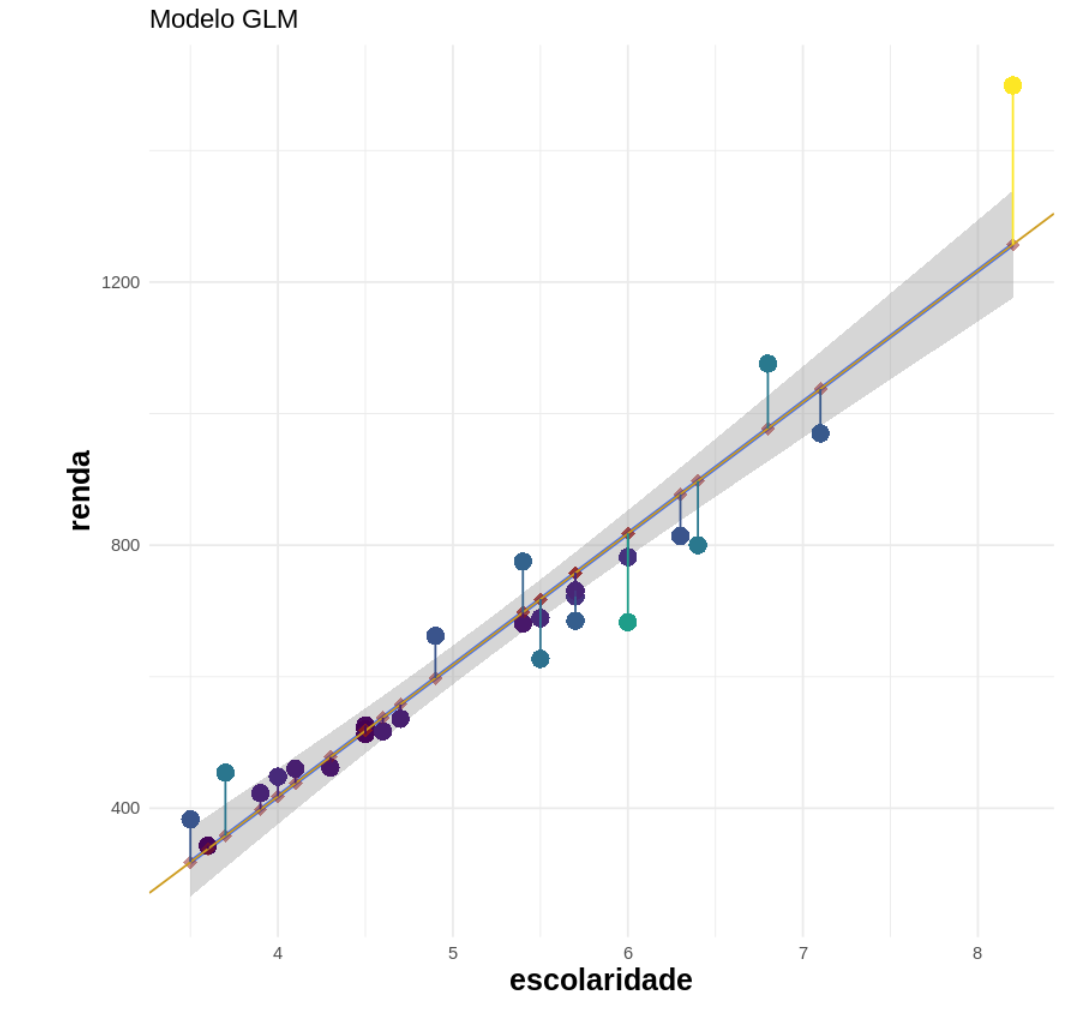
\includegraphics[scale=0.45]{2_1f_glm.png}
                     \caption{Modelo \texttt{glm} com $Gamma$.}
                     \label{fig2glm}
                \end{figure}

        \item[1.13]	Agora estime (utilize a função \texttt{predict()} ) os valores de renda para os valores de escolaridade utilizando os dois modelos (\texttt{lm()} e \texttt{glm()}) e plote os gráficos com as curvas. Mostre no mesmo gráfico os valores observados em preto, preditos do \color{red}modelo 1 em vermelho\color{black}, e preditos no \color{green} modelo 2 em verde\color{black}.( utilize as funçoes \texttt{plot()}, \texttt{points()} e \texttt{points()})\\
        \textbf{Código}:
            \begin{lstlisting}
predicao <- data.frame(escolaridade=seq(from = 0 , 
                                        to = 10 , 
                                        by = 0.25))
predicao$rendalin <- predict(modelo.lin,predicao, type='response')
predicao$rendaglm <- predict(modelo.glm,predicao, type='response')
predicao$rendagll <- predict(modelo.gll,predicao, type='response')
predicao$rendagin <- predict(modelo.gin,predicao, type='response')
predicao$rendagil <- predict(modelo.gil,predicao, type='response')
reta <- coefficients(modelo.lin)
reta <- coefficients(modelo.lin)
ggplot(mec,
       aes(x=escolaridade, y=renda), 
       color="Gray",
       ylim=c(200,1600), 
       xlim=c(0,9),  
       show.legend = FALSE) +
    expand_limits(x=c(0,12), 
                  y=c(0, 2000))+
    geom_abline(intercept = reta[1], 
                slope=reta[2], 
                col="darkgrey") +
    geom_line(aes(x= escolaridade, 
                  y=modelo.lin$fitted.values), 
              col = "red", 
              size=1,  
              alpha=0.5) +
    geom_line(aes(x= escolaridade, 
                  y=modelo.glm$fitted.values), 
              col = "green1", 
              size=1,  
              alpha=0.5) +
    geom_line(aes(x= escolaridade, 
                  y=modelo.gll$fitted.values), 
              col = "green4", 
              size=1,  
              alpha=0.5) +
    geom_line(aes(x= escolaridade, 
                  y=modelo.gin$fitted.values), 
              col = "yellow2", 
              size=1,  
              alpha=0.5) +
    geom_line(aes(x= escolaridade, 
                  y=modelo.gil$fitted.values), 
              col = "yellow4", 
              size=1,  
              alpha=0.5) +
    theme_minimal() +
    theme(axis.title = element_text(color="black", 
                                    size=15, 
                                    face=2))+
    scale_color_viridis() +
    geom_point(shape = 16, 
               size = 2, 
               show.legend = FALSE, 
               alpha=0.5) +
    ggtitle("Comparativo dos modelos") 
            \end{lstlisting}
            \textbf{Resposta}: Uma visualização dos dados e modelos é apresentada na Figura \ref{fig2all}. Nota: em \color{red}vermelho \color{black}a reta representando o modelo linear \texttt{lm}, em tons de \color{green}verde\color{black}, o \texttt{glm()}, sendo o claro do \textit{Gamma()} e o mais escuro o \textit{Gamma( link='log'}. Já os tons de \color{yellow}amarelo \color{black}são a visualizaçao da \textit{gaussiana invertida} (clara) e \textit{gaussiana invertida} com escala em log (escura), para curiosidade e ajudar a ilustrar o uso dos modelos.
                \begin{figure}[h!tb]
                     \centering
                     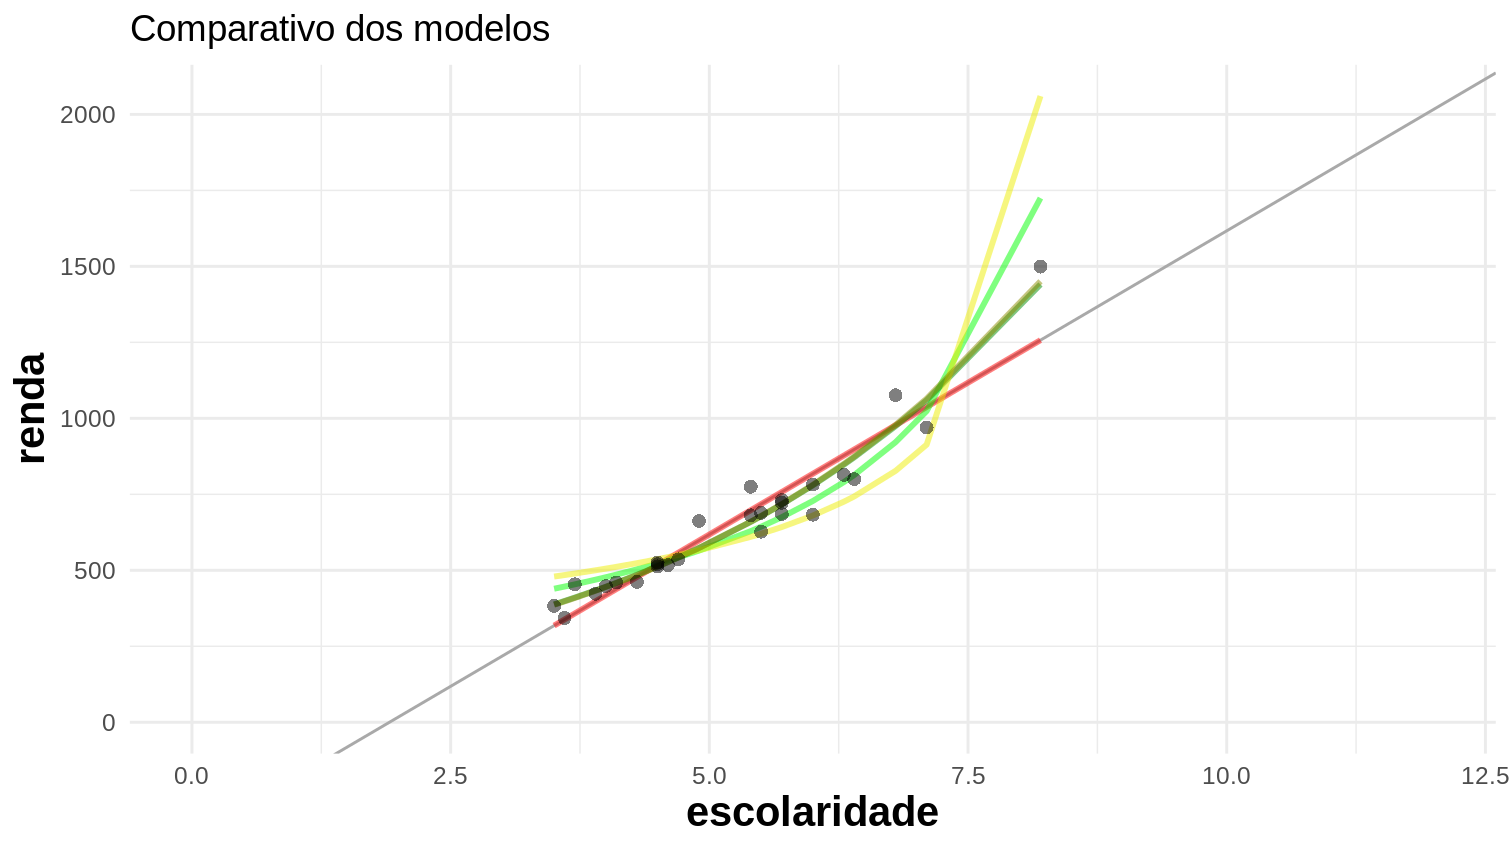
\includegraphics[scale=0.75]{2_1g_all.png}
                     \caption{Comparativo entre os modelos.}
                     \label{fig2all}
                \end{figure}
        \item[1.14] Compare os modelos com a função AIC e informe qual modelo você escolhe e por que?\\
        \textbf{Código}:
            \begin{lstlisting}
print(data.frame(
modelos = c('Linear', 
            'Gamma', 'Gamma-Log', 
            'GaussInv', 'GaussInv-Log'),
aic = c(AIC(modelo.lin),        
        AIC(modelo.glm), AIC(modelo.gll),
        AIC(modelo.gin), AIC(modelo.gil)), 
verossimilhança = c(logLik(modelo.lin), 
                   logLik(modelo.glm),logLik(modelo.gll),
                   logLik(modelo.gin),logLik(modelo.gil)))
)
# saida
  modelos      aic verossimilhança
1       Linear 315.2632       -154.6316
2        Gamma 304.9130       -149.4565
3    Gamma-Log 288.1337       -141.0669
4     GaussInv 326.4785       -160.2392
5 GaussInv-Log 288.9597       -141.4798
            \end{lstlisting}
        \textbf{Resposta}: O modelo que escolheria seria o modelo \textit{Gamma-Log}, que melhor se ajusta e com resíduos mais próximos, vide a maior verossimilhança e menor \texttt{AIC}. Em caso de não usar os ajustes com \textit{log}, o próprio \textit{Gamma} seria o escolhido (segundo os mesmos critérios). O gráfico da saída do \texttt{hnp()} mostra que a \textit{Normal Q-Q} tem os dados mais próximos do eixo e mais concentrado no centro, como mostra de melhor ajuste conforme dados observados. 
    \end{enumerate}
    % \newpage

\subsubsection{Exercício 2}

    \item Encontre uma base de dados de sua preferência, caso não possua alguma há várias disponíveis no \url{https://www.kaggle.com/datasets} e \url{http://dados.gov.br/dataset}, e faça uma análise de regressão ou \textit{forecast} sobre alguma informação que lhe pareça importante. Atenção que todas as \textbf{análises dos resultados e gráficos devem ser exibidas, comentadas e descritas} abaixo.\\
    
    \textbf{Resposta}:\\
    A base de dados escolhida foi a da AAVSO\footnote{\textit{American Association of Variable Star Observers}, url: \url{https://aavso.org}.} (buscada através do portal \textit{Simbad}\footnote{A busca foi feita na url: \url{https://simbad.u-strasbg.fr/simbad/sim-id?Ident=alpha\%20Orionis}.}. O tema de busca foi o caso da estrela Betelgeuse no trimestre final de 2019 e início de 2020.\\
                \begin{figure}[h!tb]
                     \centering
                     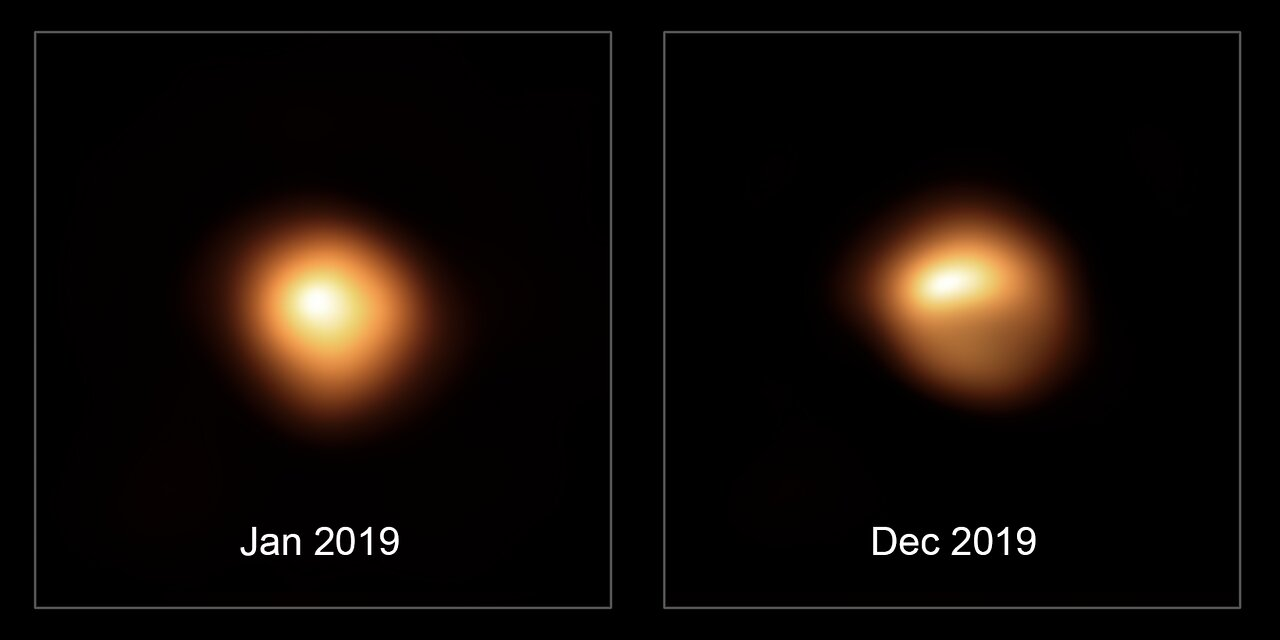
\includegraphics[scale=0.35]{2_2_ao.jpg}
                     \caption{Fotos do inicio e fim de 2019: Betelgeuse ($\alpha$ \textit{Orinidis}).}
                     \label{fig2all}
                \end{figure}
    A estrela Betelgeuse sempre teve o comportamento oscilativo da sua luminância em ciclos $~ 5.9$ anos\footnote{Updates on the "Fainting" of Betelgeuse. url: \url{https://www.astronomerstelegram.org/?read=13365}}. No final de 2019, astrônomos Universidade Villanova, viram que esta estava diminuindo a luminância por uma fator maior que o comum\footnote{EVOLUTIONARY TRACKS FOR BETELGEUSE. url: \url{https://iopscience.iop.org/article/10.3847/0004-637X/819/1/7}}.\\
    Portanto aí estava um tema interessante para avaliar os dados e testar previsões (nos momentos do ano passado e atual), além de uma previsão geral para o próximo ano.\\
    \begin{enumerate}
        \item O primeiro passo foi escolher um corte no tempo (há muitas observações). No site foi selecionado desde 2015. Após descarregado, temos os seguintes passos: analisar a base e separar as informações desejadas. Comandos:\\
        \textbf{Código}:
            \begin{lstlisting}[lang=bash]
$ wc -l aavsodata_betelgeuse.csv
    9492 aavsodata_betelgeuse.csv
$ head aavso_betelgeuse.csv
1- JD,Magnitude,Uncertainty,HQuncertainty,Band,Observer Code,
Comment Code(s),Comp Star 1,Comp Star 2,Charts,Comments,
Transfomed,Airmass,Validation Flag,Cmag,Kmag,HJD,Star Name,
Observer Affiliation,Measurement Method,Grouping Method,ADS
Reference,Digitizer,Credit
2- 2457023.54375,0.5,,,Vis.,MCPA,U,01,09,10 star,,,,Z,,,,ALF ORI,
AAVSO,STD,,,,
3- 2457023.8680,-3.084,0.050,,J,KCD,,GAMMA ORI,,13650PT,,1,,Z,
,,,ALF ORI,BAA-VSS,STD,1,,,
4- 2457023.8680,-4.076,0.050,,H,KCD,,GAMMA ORI,,13650PT,,1,,Z,
,,,ALF ORI,BAA-VSS,STD,1,,,
5- 2457024.3,0.3,,,Vis.,SPAO,,03,17,680301,,,,Z,,,,ALF ORI,UAI,
STD,,,,
        \end{lstlisting}
        \item O arquivo contém \texttt{Magnitude} (observação que nos interessa), além da coluna \texttt{JD} (que após pesquisas em sites de astronomia, significa \textit{Julian Date} - representação de datas usada na comunidade astronômica).\\
        Cabe identificar que há muitos dados além do que gostaríamos, nos interessa a banda da luz visível, para deixar uma informação de mesma característica. Assim a coluna \texttt{Band} nos ajuda a filtar as informações que queremos. Portanto, para filtrar antes de carregar no \texttt{R}, vamos tratar de ``limpar'' os dados pra facilitar o uso. Assim iremos fazer 3 passos:
        \begin{enumerate}
            \item Pega as primeiras 5 colunas (até o que precisamos, \texttt{Band}):
            \begin{lstlisting}[lang=bash]
# comando pra pegar o cabeçalho:
$ head -n 1 aavsodata_original.csv | 
                       cut -d',' -f1-2 > aavso_data.csv
# (construindo o comando) pegando as colunas 5 colunas:
$ cut -d',' -f1-5 avsodata_betelgeuse.csv
            \end{lstlisting} 
            \item Após isso, vamos filtrar somente as observações visuais (\texttt{Vis.}) - e com isso podemos descartar essa coluna:
            \begin{lstlisting}[lang=bash]
# selecionando somente o que houver Vis:
$ cut -d',' -f1-5 avsodata_betelgeuse.csv | grep 'Vis'
            \end{lstlisting}    
            \item Por último teremos somente as duas primeiras colunas (data e magnitude):\\
            \begin{lstlisting}[lang=bash]

# do resultado, pega somente a primeiras 2 colunas:
$ cut -d',' -f1-5 avsodata_betelgeuse.csv | grep 'Vis' |
                         cut -d',' -f1-2 >> aavso_data.csv
            \end{lstlisting}    
        \end{enumerate}
        Ao final deste passo, ficam-se com 7645 pontos de observação.
    \end{enumerate}
    \item Com isso, iniciamos os trabalhos no \textit{R}, carregando as bibliotecas e os dados em um \textit{dataframe}:
        \begin{lstlisting}[lang=R]
# biblioteca de gráficos
library(ggplot2)
# bibliotecas para manipulação de datas e funções Astronomicas
library(astrolibR)
library(astroFns)
# manipular dataframes
library(data.table)
aavso_data <- read.csv2("aavso_data.csv", sep=",")
head(aavso_data)
        \end{lstlisting}   
    \item Após carregar os dados, vamos limpar os dados \texttt{NA} (\textit{Not Available}), que por algum motivo afetam a coluna \textit{magnitude}. Vamos aproveitar (pra uso no futuro) e criar uma coluna \texttt{dia}, para termos as datas conforme relativas ao primeiro dia da base.
        \begin{lstlisting}
Dados_preNA <- data.frame(date=as.Date(jd2ymd(as.double(aavso_data$JD))))
Dados_preNA$magnitude <- as.double(aavso_data$Magnitude)
Dados = Dados_preNA[complete.cases(Dados_preNA),]
Dados$dia <- as.numeric(Dados$date-min(Dados$date))
        \end{lstlisting}    
    \item Após este passo, ficam 7634 pontos de observação (9 \texttt{NA}s foram removidos). Com isso vamos ver um resumo dos dados:
         \begin{lstlisting}
summary(Dados)
        \end{lstlisting}  
    \item Vamos ver como ficam os pontos observados no gráfico:
        \begin{lstlisting}
ggplot(Dados,
       aes(x=date,     
           y=magnitude,      
           color=(magnitude),       
           alpha=0.5), 
       ylim=c(-10,14)) +

  geom_point(shape = 16, 
             size = 2, 
             show.legend = FALSE, 
             alpha=0.6) +
  theme_minimal() +
  theme(axis.title = element_text(color="black", 
                                  size=15, 
                                  face=2))
        \end{lstlisting}   
        \begin{figure}[h!tb]
             \centering
             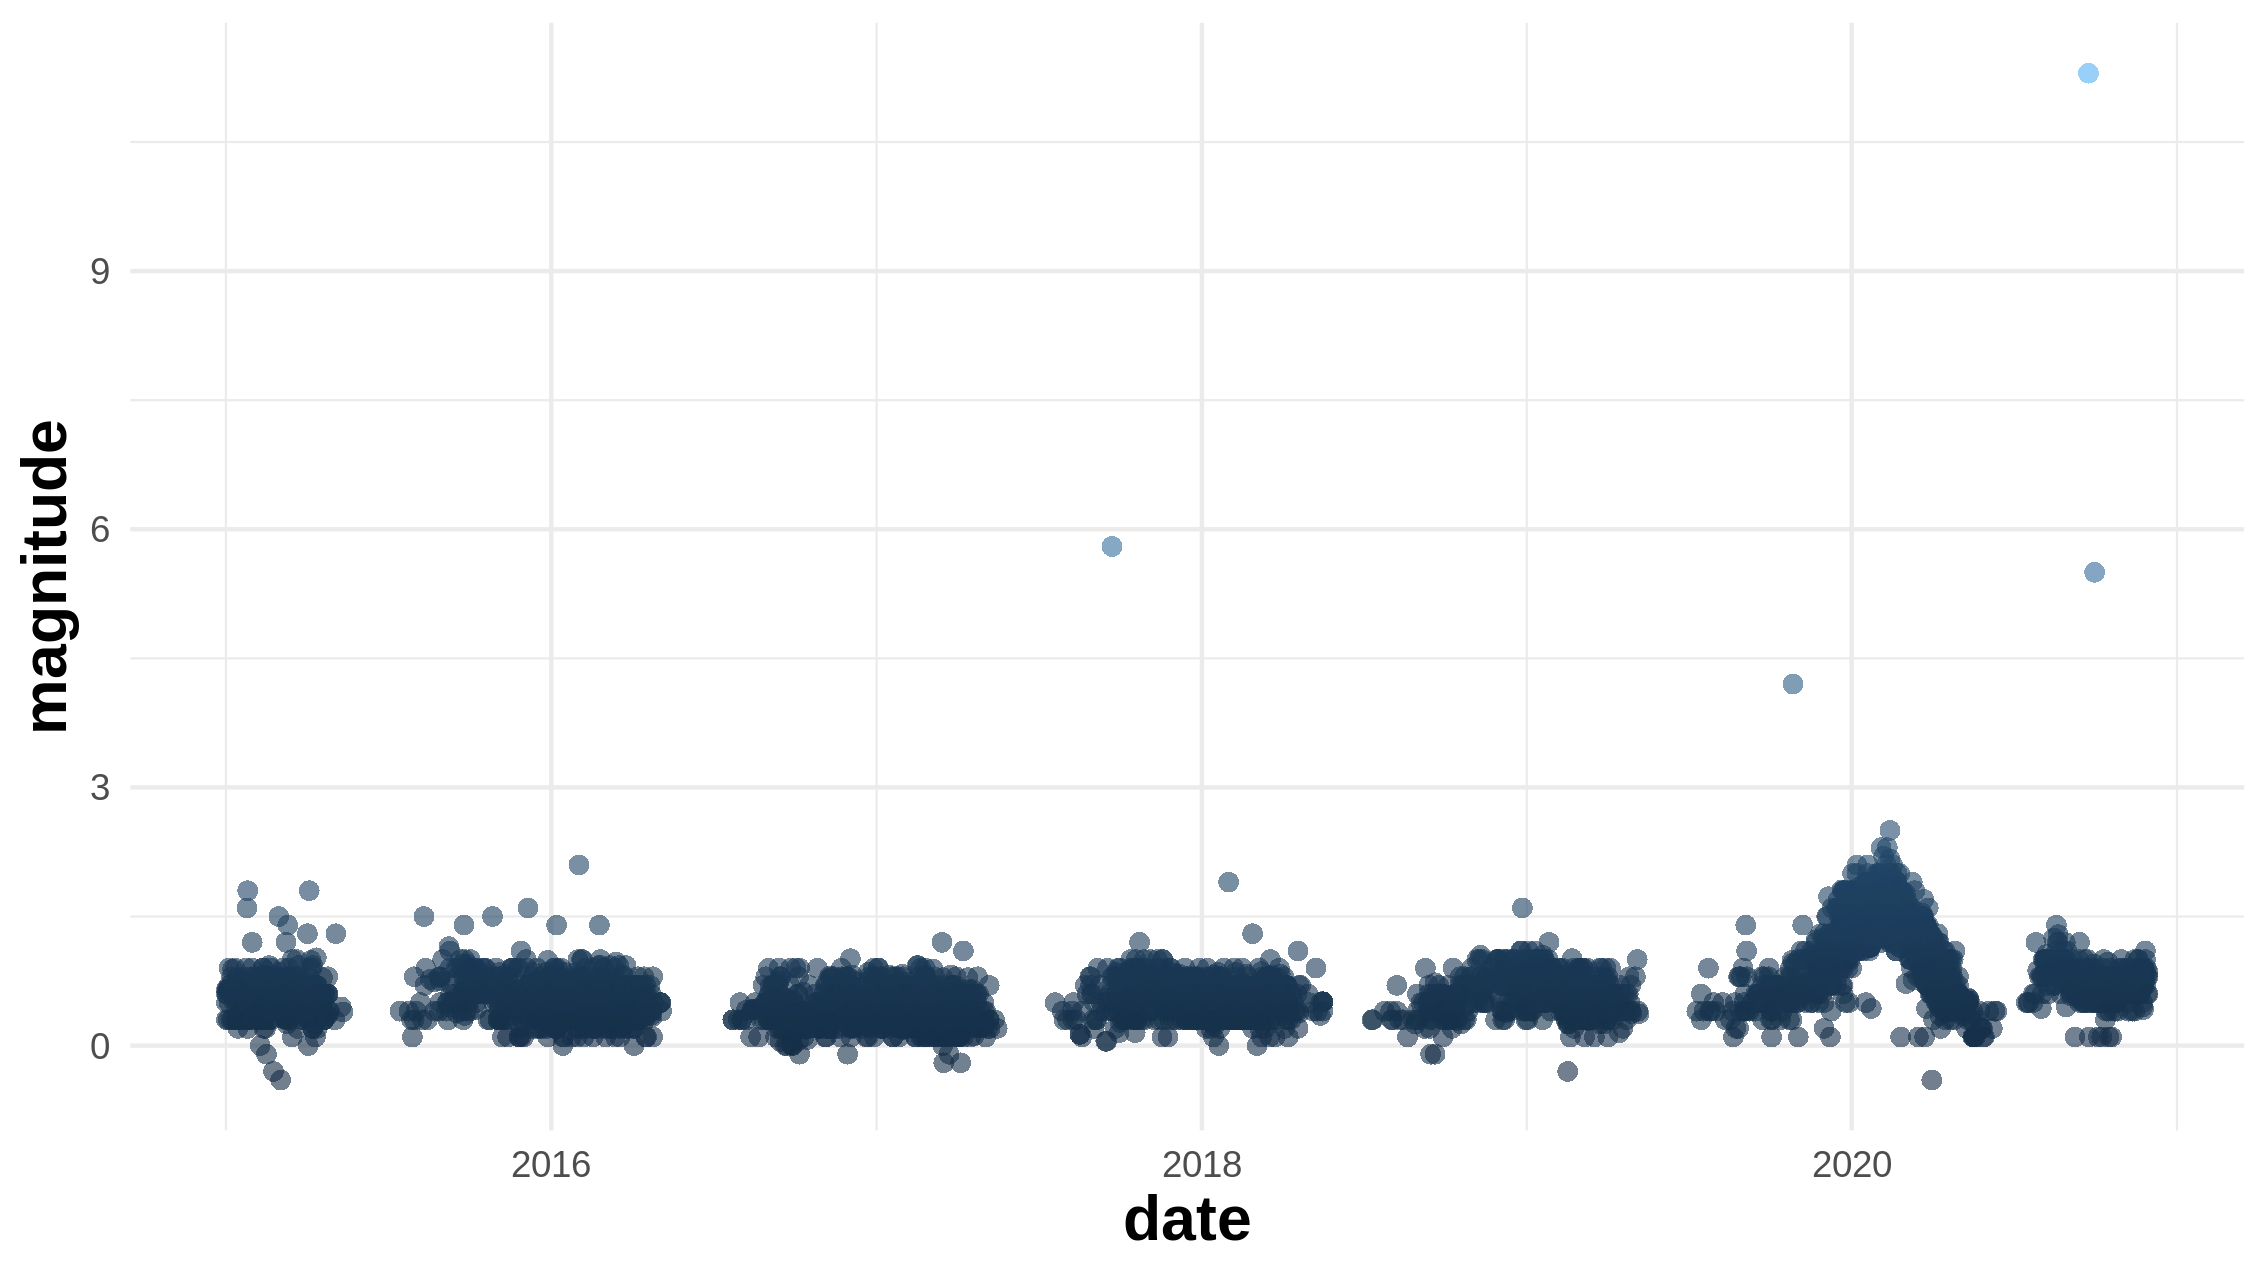
\includegraphics[scale=0.75]{2_2_00.png}
             \caption{Observações visuais da Betelgeuse ($\alpha$ \textit{Orinidis}).}
             \label{fig2obs}
        \end{figure}
    \item Na Figura \ref{fig2obs} observa-se que há alguns valores discrepantes (que não fazem sentido). Como são 4 pontos, vamos removê-los do data.frame:
        \begin{lstlisting}
outlierReplace = function(dataframe, cols, rows, newValue = NA) {
    if (any(rows)) {
        set(dataframe, rows, cols, newValue)
    }
}
outlierReplace(Dados, c("magnitude"), which(Dados$magnitude > 3), NA)
        \end{lstlisting}  
    Plotando o gráfico sem os 4 pontos discrepantes (com total agora de 7630):
        \begin{figure}[h!tb]
             \centering
             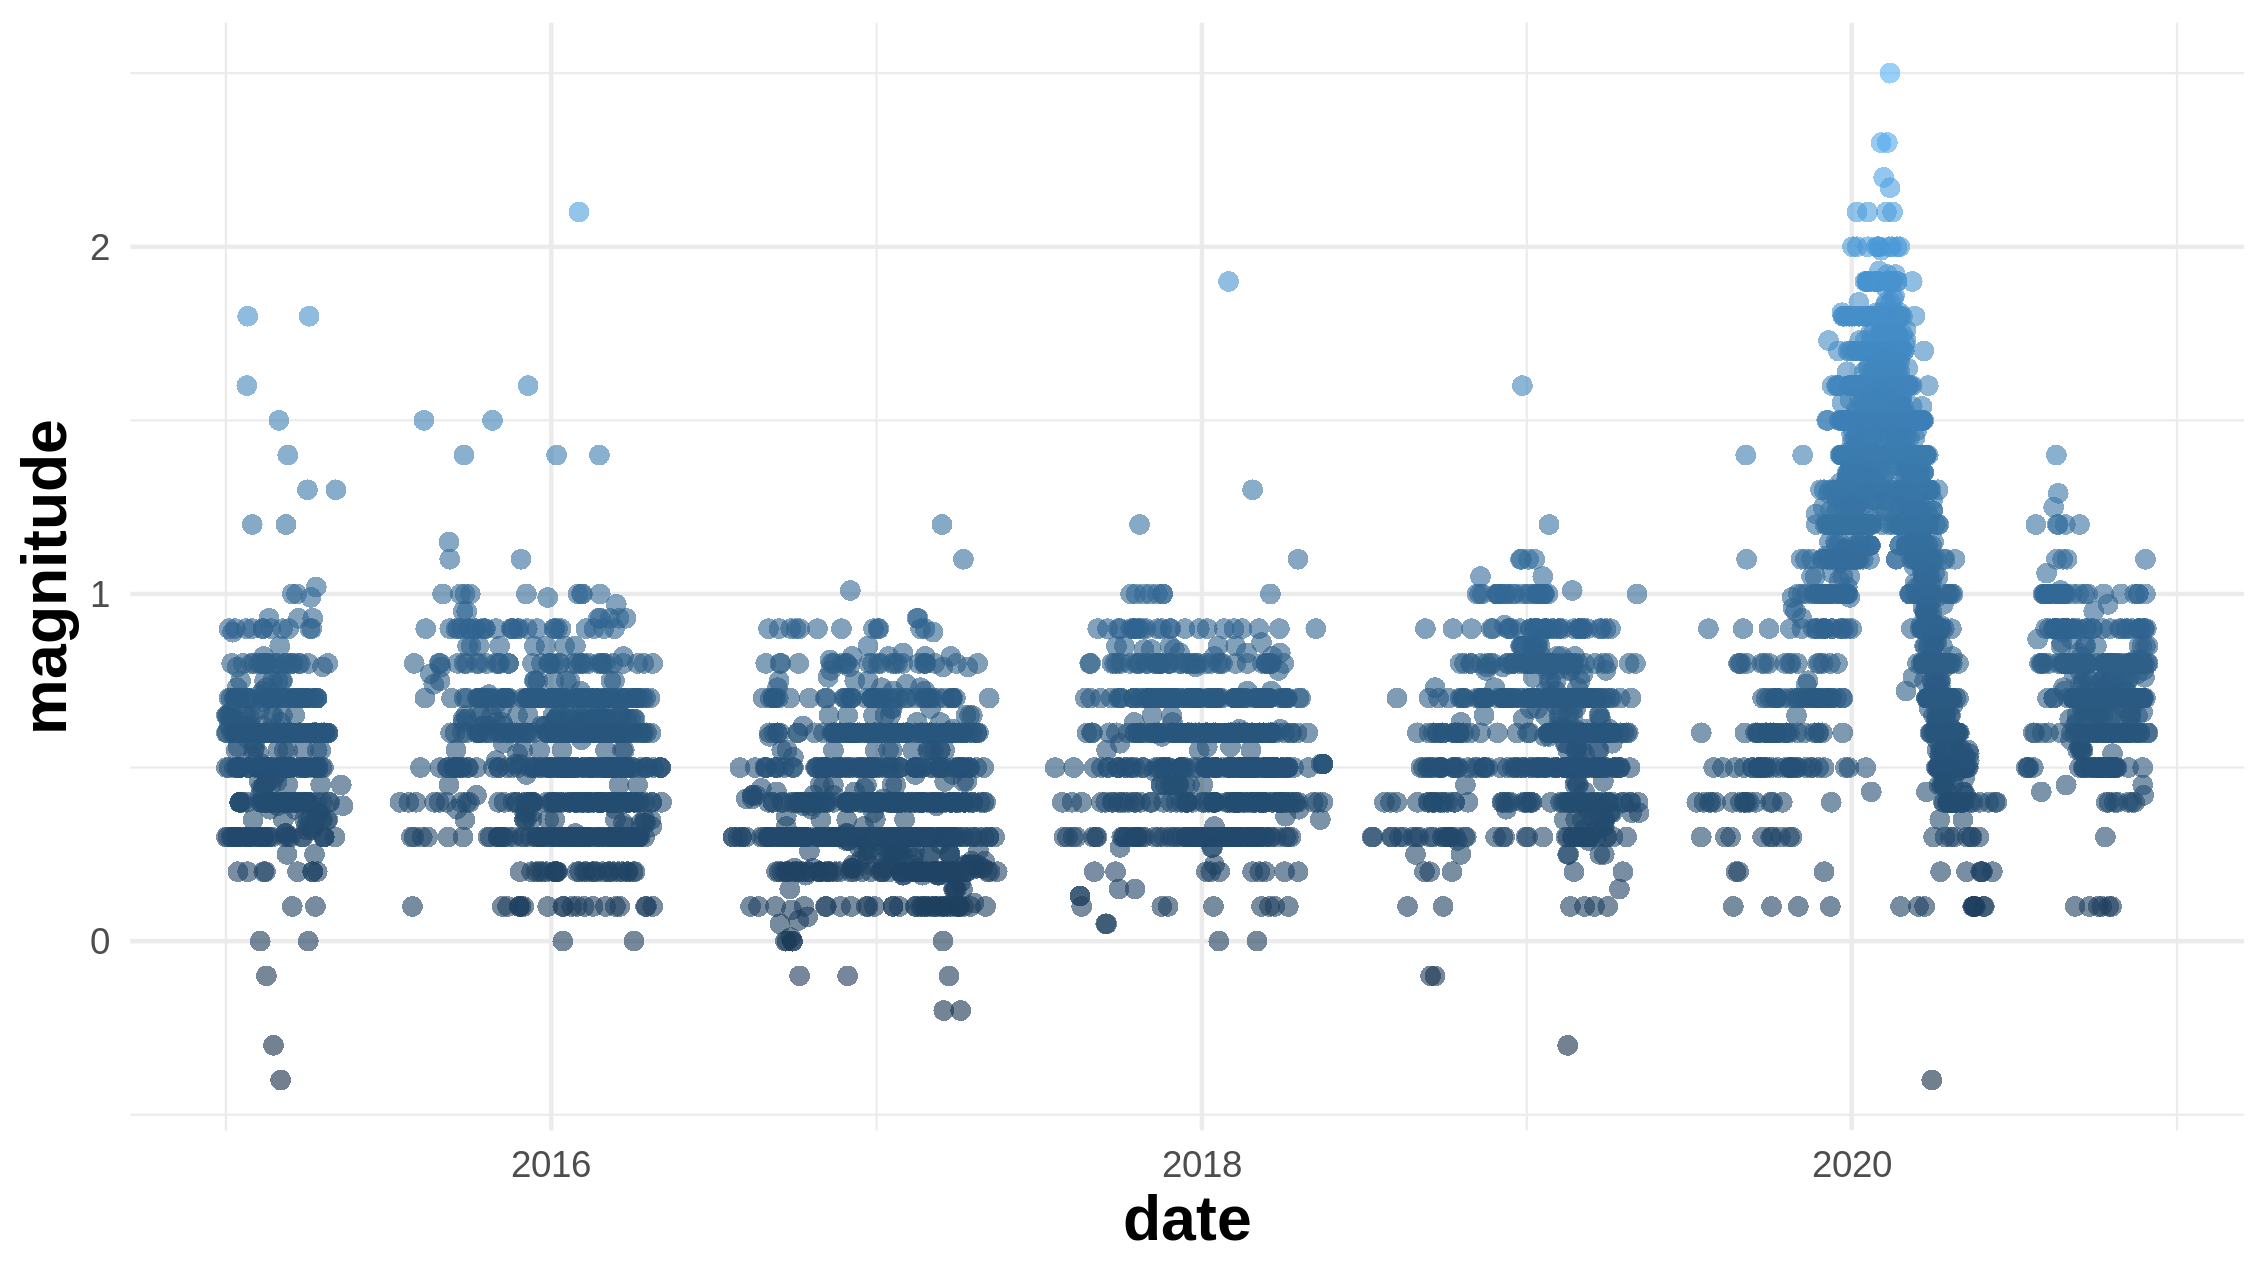
\includegraphics[scale=0.75]{2_2_01.png}
             \caption{Observações visuais sem valores discrepantes.}
             \label{fig2obs}
        \end{figure}
    \item Aplicando um modelo linear, temos:
        \begin{lstlisting}
# # testando um modelo linear
ggplot(Dados,
       aes(x=date,     
           y=magnitude))+
  geom_line(aes(x=date,     
           y=magnitude,            
           color="lightblue",
           alpha=0.2), 
           show.legend = FALSE) + 
  geom_smooth(method = "lm", 
              se = TRUE,
              show.legend = FALSE) + 
  theme_minimal() +
  theme(axis.title = element_text(color="black", 
                                  size=15, 
                                  face=2))

ggsave("2_2_02.png",
          plot=last_plot(),
      scale = 1:1,
      width=192,
      height=108,
      units="mm",
      dpi=300)
        \end{lstlisting} 
        \begin{figure}[h!tb]
             \centering
             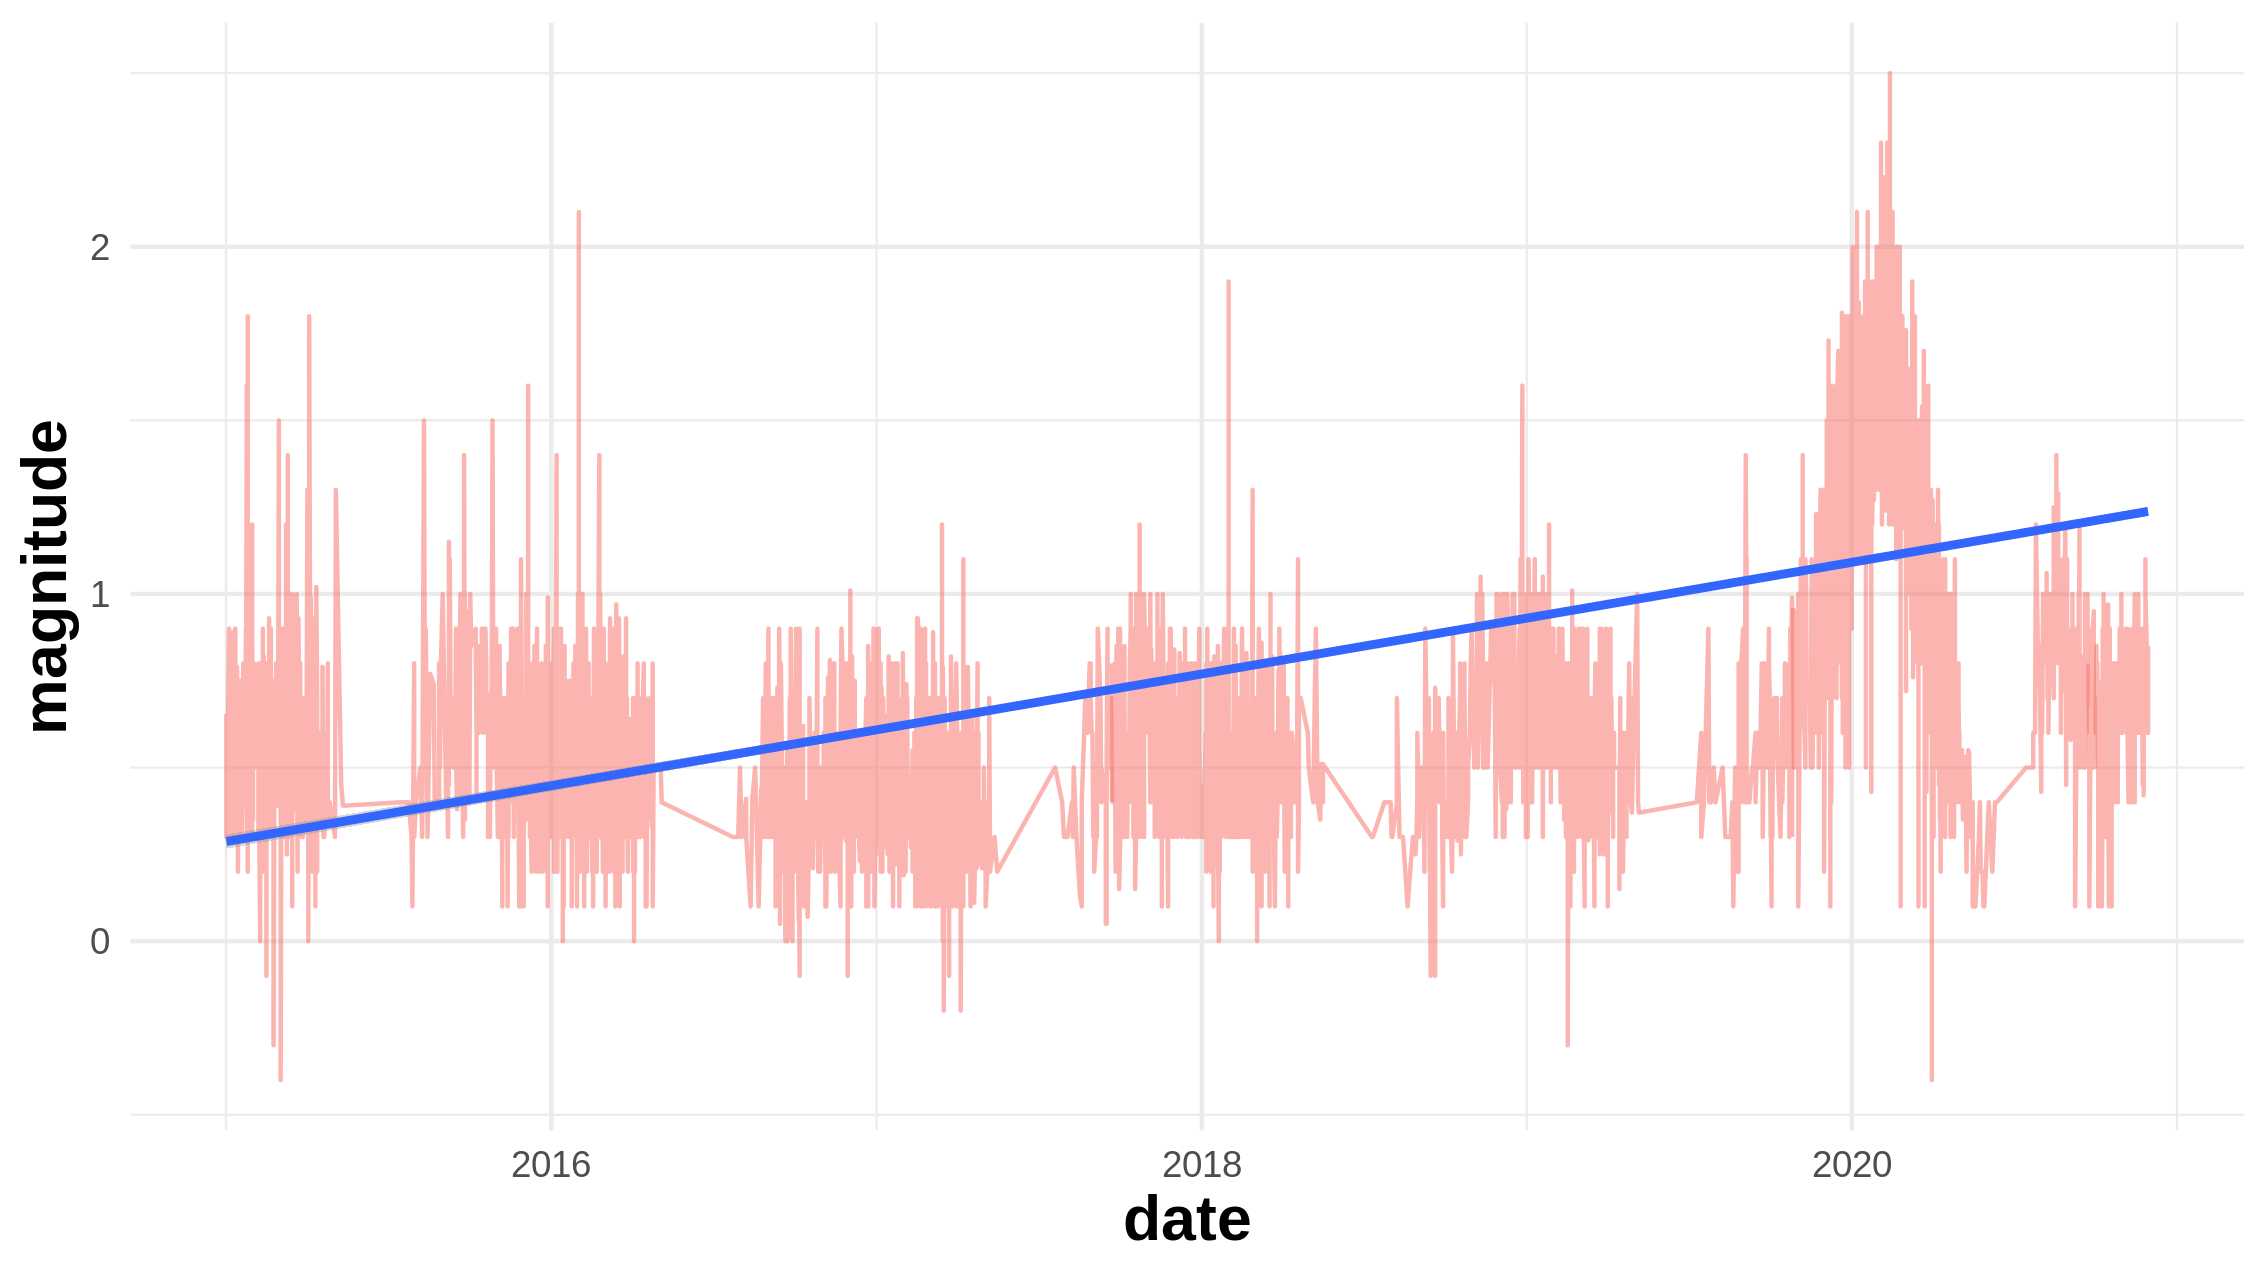
\includegraphics[scale=0.75]{2_2_02.png}
             \caption{Modelo Linear.}
             \label{fig2lin}
        \end{figure}
    \item Como observou-se na Figura \ref{fig2lin}, o modelo linear é muito reduzido para a características dos dados, ficando muito aquém do que se esperaria. Assim, vale testar a biblioteca \texttt{forecast}.
        \begin{lstlisting}
tsData <- ts(data=magnitude, 
             frequency=365, 
             start=c(2015,1), 
             end=c(2020,12))
htt1 <- HoltWinters(tsData, 
                    gamma=FALSE, 
                    l.start = sbux[1])
plot(htt1)
prev_htt1 <- forecast(htt1, h=60)
plot(prev_htt1)
        \end{lstlisting}
        \begin{figure}[h!tb]
             \centering
             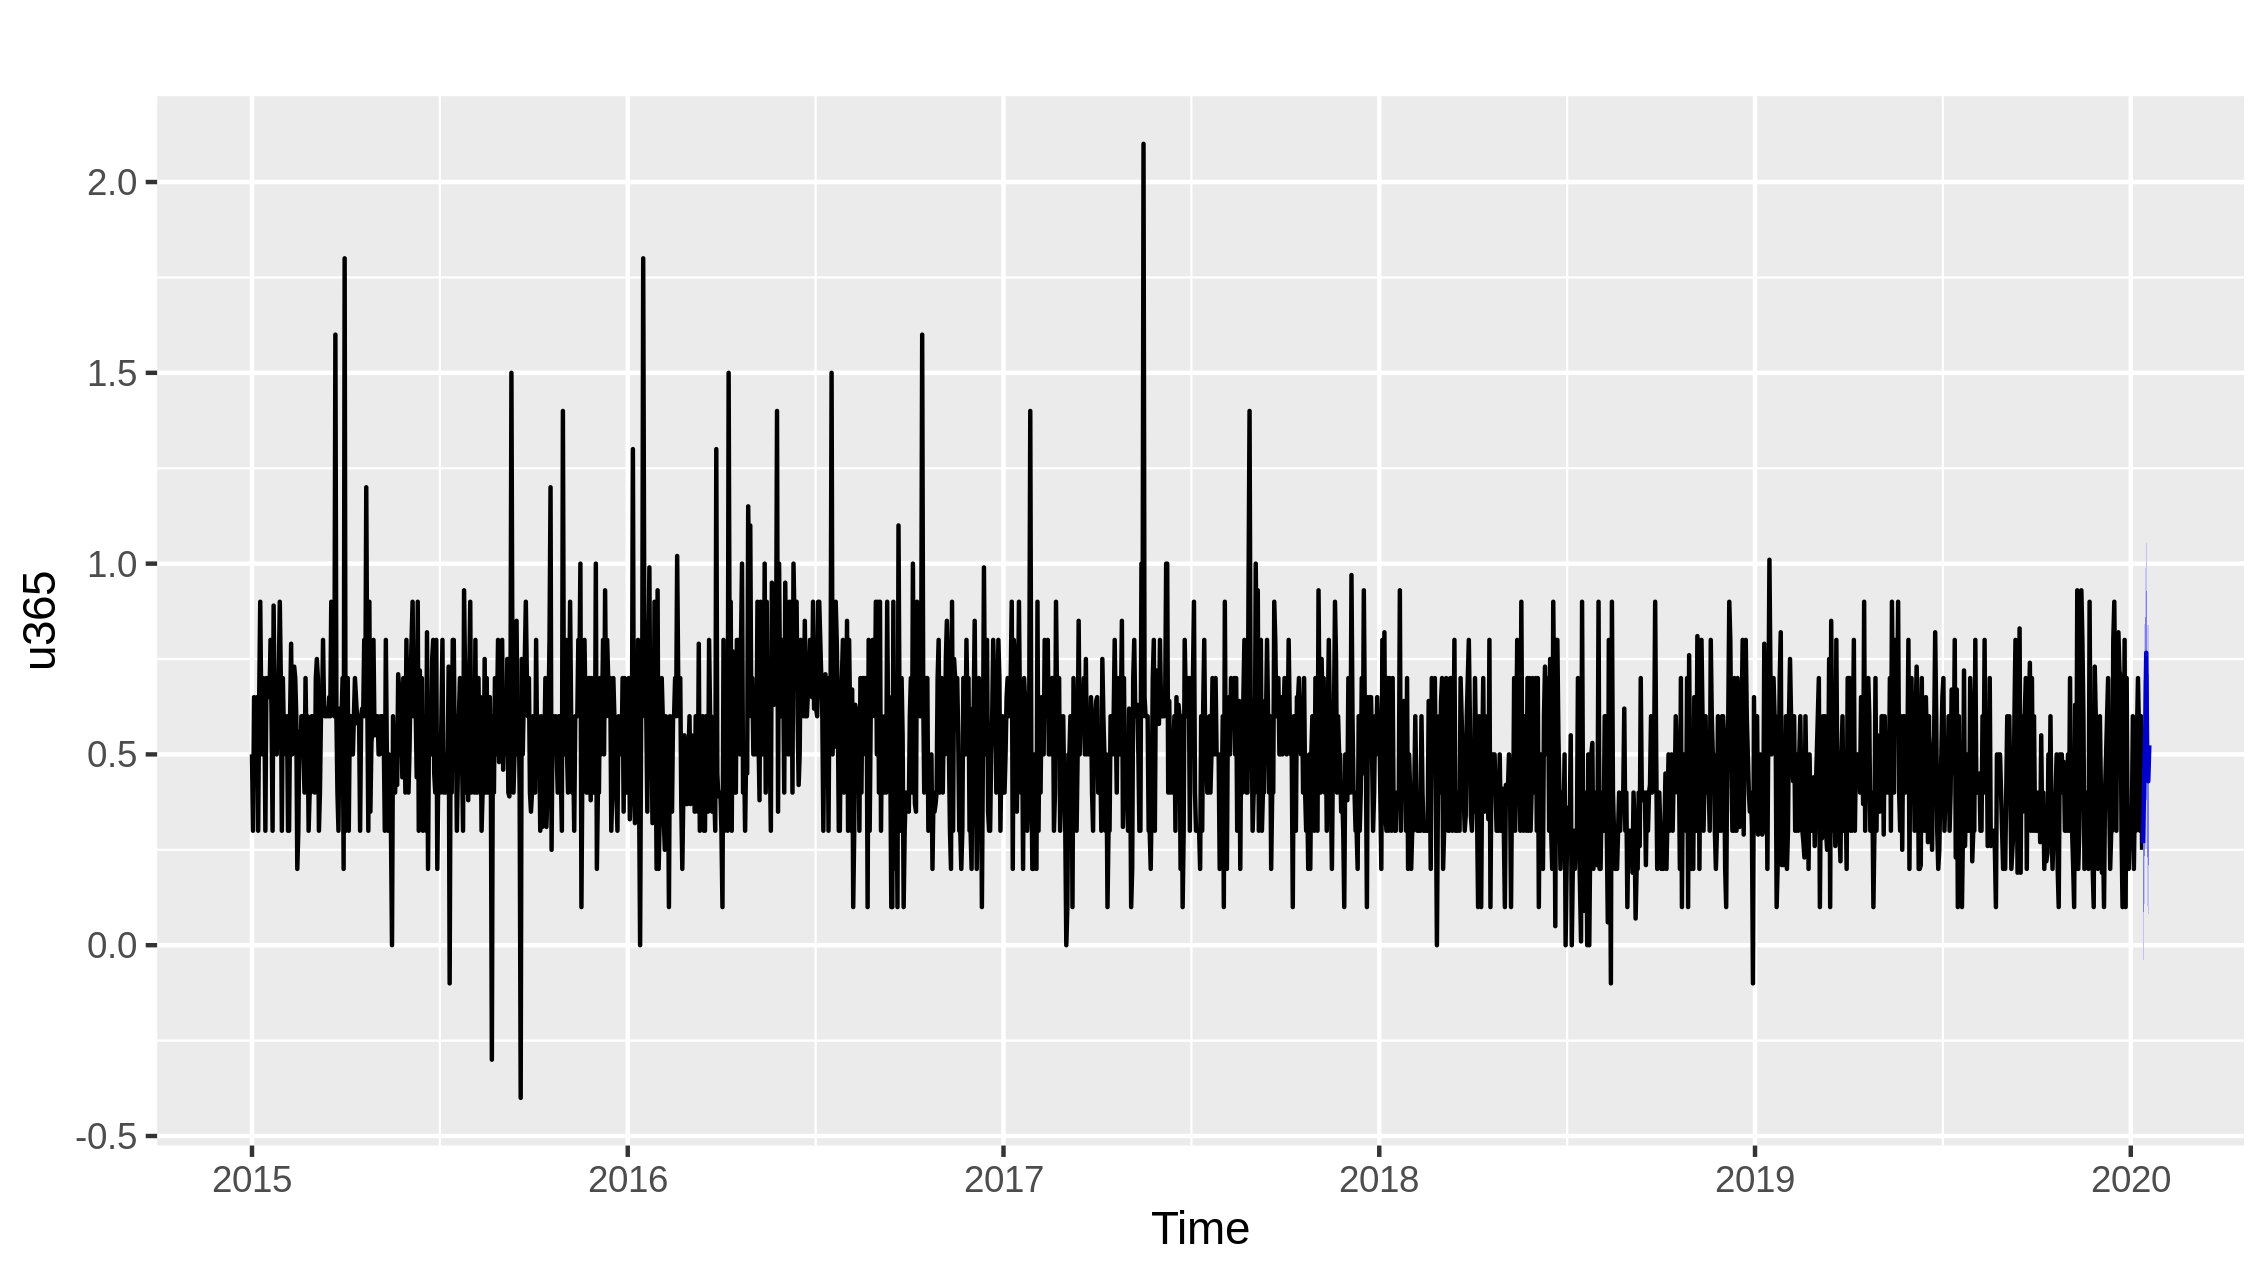
\includegraphics[scale=0.75]{2_2_03a.png}
             \caption{\textit{Holt-Winters} observado/ajustado.}
             \label{fig2hw01}
        \end{figure}
        \begin{figure}[h!tb]
             \centering
             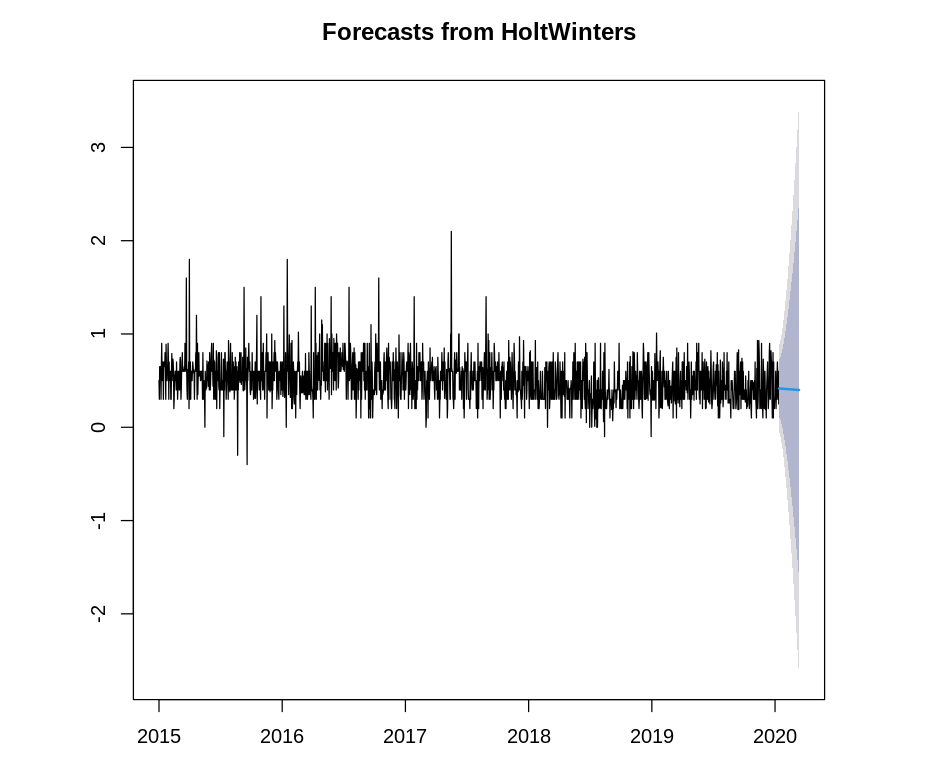
\includegraphics[scale=0.75]{2_2_03b.png}
             \caption{Previsão com \textit{Holt-Winters} para 60 dias.}
             \label{fig2hw02}
        \end{figure}
            \item Na Figura \ref{fig2hw01}, é mostrada a função de \textit{Holt-Winters} conforme o observado e os dados ajustados. Já na Figura \ref{fig2hw02}, tem-se os dados observados e a previsão para 60 dias.
        \begin{lstlisting}
htt2 <- HoltWinters(tsData)
prev_htt2 <- forecast(htt2, h=365)
plot(prev_htt2)
        \end{lstlisting} 
            \begin{figure}[h!tb]
             \centering
             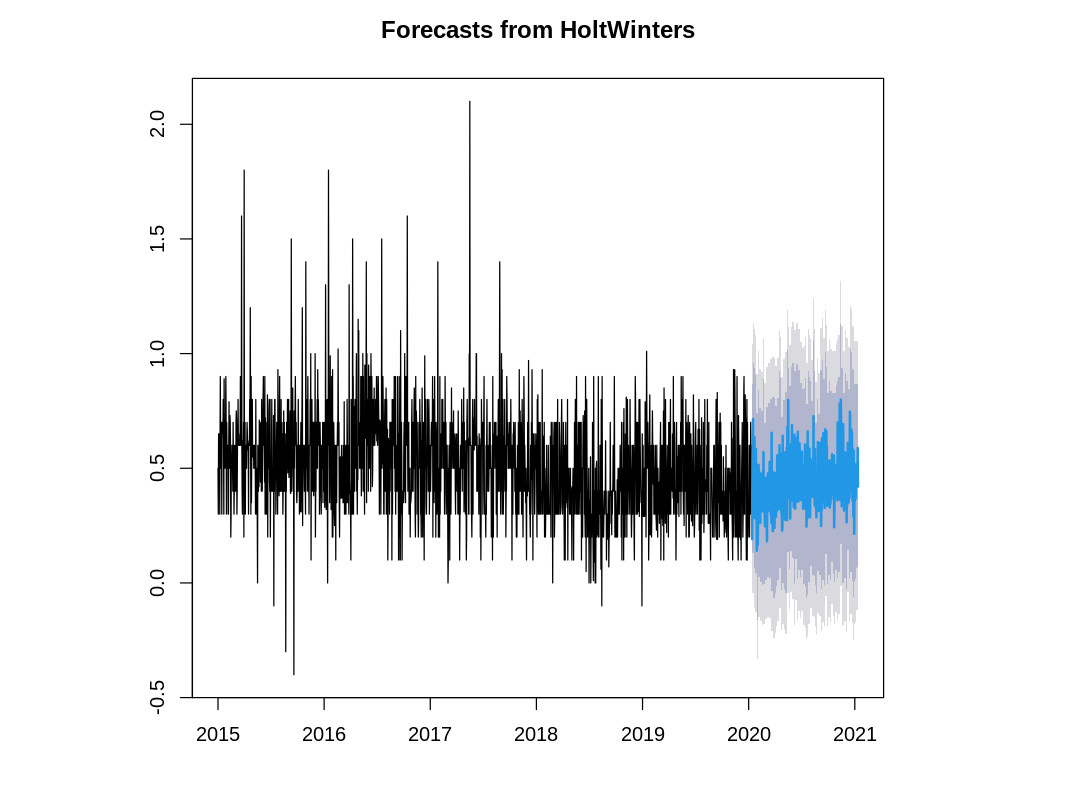
\includegraphics[scale=0.75]{2_2_04.png}
             \caption{Previsão com \textit{Holt-Winters} para 1 ano.}
             \label{fig204}
            \end{figure}
                \item Observa-se que a previsão pra um ano (Figura \ref{fig204} é bem mais ajustada ao comportamento dos dados.
        \begin{lstlisting}
m <- HoltWinters(tsData)
p <- predict(m, 60, prediction.interval = TRUE)
plot(m,p)
        \end{lstlisting}    
        \begin{figure}[h!tb]
             \centering
             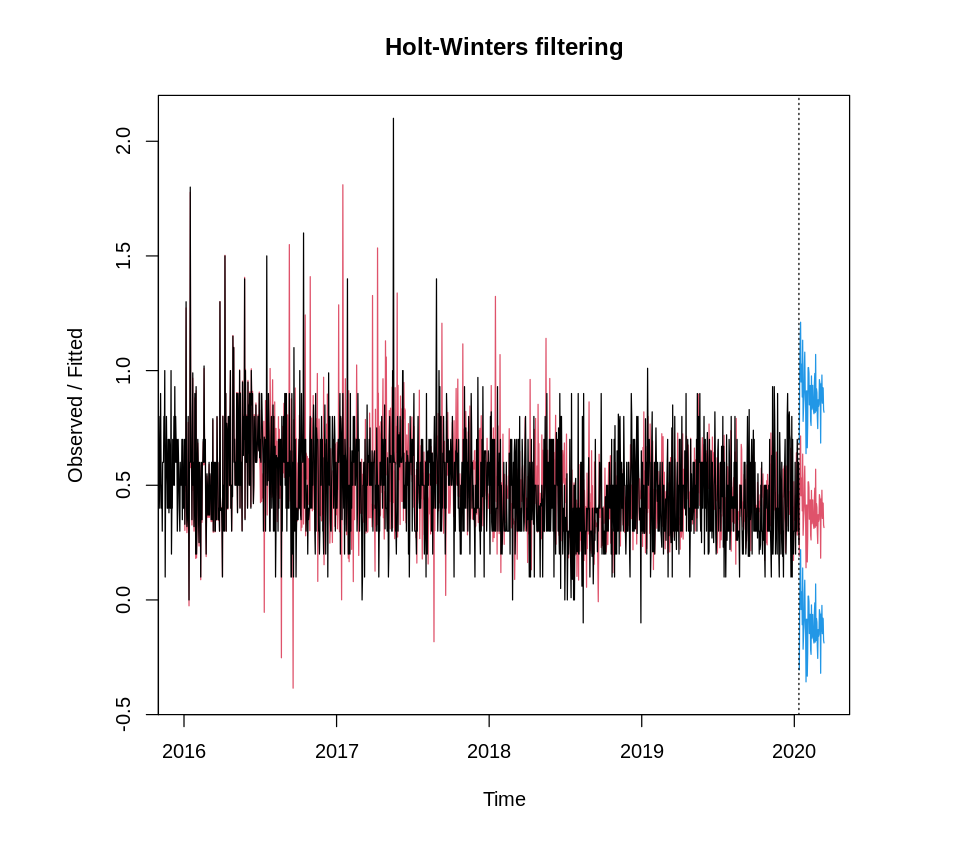
\includegraphics[scale=0.75]{2_2_05.png}
             \caption{Previsão para 60 dias, com intervalo destacado.}
             \label{fig205}
        \end{figure}
     \item Já na Figura \ref{fig205}, é outra opção de previsão com destaques para os intervalos superiores e inferiores.
\end{enumerate}

\subsubsection{Comentários}

Series temporais tem inúmeros usos e fazem parte do nosso dia-a-dia. O maior desafio, sempre mencionado por quem trabalha com dados, é a obtenção dos dados, limpeza e ajustes dos mesmos. Previsão e séries temporais nos ajudam a ter parâmetros de comportamentos futuros (baseado no passado) dos dados observados. Um ponto que vale destacar é o domínio do conhecimento dos dados, pois desde a aquisição, tratamento e seleção do modelo, se faz necessário ter um conhecimento mínimo das informações envolvidas.\\
No caso específico do exemplo, temos que alguns modelos (como o linear) não auxiliam nas previsões. Modelos que levam em consideração sazonalidades e tendencias acabam sendo mais ajustados para o nosso exemplo, a magnitude da Betelgeuse.  

\end{document}


